\documentclass{article}

\PassOptionsToPackage{numbers,sort&compress}{natbib}
\usepackage[preprint]{neurips_2021}
\usepackage[utf8]{inputenc}
\usepackage[T1]{fontenc}
\usepackage{hyperref}
\usepackage{url}
\usepackage{booktabs}
\usepackage{microtype}
\usepackage[table]{xcolor}
\usepackage{graphicx}
\usepackage{subcaption}
\usepackage{multirow}
\usepackage{array}
\usepackage{makecell}
\usepackage{adjustbox}
\usepackage{enumitem}
\usepackage{algorithm}
\usepackage{algpseudocode}
\usepackage{amsmath}
\usepackage{amssymb}
\usepackage{amsfonts}
\usepackage{amsthm}
\usepackage{mathtools}
\usepackage{bm}
\usepackage{caption}
\usepackage{wrapfig}
\usepackage{float}

\title{CDA: Post-hoc Domain Generalization by Distributional Canalization}

\author{
Jayden Jeong\\
Math, Science, and Technology Center (MSTC)\\
Paul Laurence Dunbar High School\\
Lexington, Kentucky, USA\\
\texttt{jayden.w.jeong@gmail.com}
\And
Vijayan K. Asari\\
School of Engineering, Department of Electrical and Computer Engineering\\
University of Dayton\\
Vision Lab, Center of Excellence for Computational Intelligence and Machine Vision\\
Dayton, Ohio, USA\\
\texttt{vasari1@udayton.edu}
}

\newif\ifsubmissionmode
\ifdefined\submissionmodeflag
  \submissionmodetrue
\else
  \submissionmodefalse
\fi

\newcommand{\placeholderguard}[1]{%
  \ifsubmissionmode
    \PackageError{cda_final_v2}{Provisional red content remains in submission mode}{Remove all provisional red content before building in submission mode.}%
  \else
    {\color{red!70!black}#1}%
  \fi
}
\newcommand{\prov}[1]{\placeholderguard{#1}}
\newcommand{\provnum}[1]{\placeholderguard{#1}}
\newcommand{\provcaption}[1]{\placeholderguard{#1}}
\newcommand{\data}[1]{\textsc{#1}}

\newtheorem{theorem}{Theorem}[section]
\newtheorem{proposition}[theorem]{Proposition}
\newtheorem{lemma}[theorem]{Lemma}
\newtheorem{corollary}[theorem]{Corollary}
\newtheorem{assumption}[theorem]{Assumption}
\theoremstyle{definition}
\newtheorem{definition}[theorem]{Definition}
\newtheorem{remark}[theorem]{Remark}

\newcommand{\RR}{\mathbb{R}}
\newcommand{\EE}{\mathbb{E}}
\newcommand{\cA}{\mathcal{A}}
\newcommand{\cB}{\mathcal{B}}
\newcommand{\cD}{\mathcal{D}}
\newcommand{\cH}{\mathcal{H}}
\newcommand{\cS}{\mathcal{S}}
\newcommand{\simplex}{\Delta}
\newcommand{\one}{\mathbf{1}}
\newcommand{\eps}{\varepsilon}
\newcommand{\cda}{\textup{\textsc{CDA}}}
\newcommand{\vsc}{\textup{\textsc{VSC}}}
\newcommand{\piv}{\textup{\textsc{CDA-Piv}}}
\newcommand{\bd}{\textup{\textsc{CDA-BD}}}
\newcommand{\erm}{\textup{\textsc{ERM}}}
\newcommand{\swad}{\textup{\textsc{SWAD}}}
\newcommand{\diwa}{\textup{\textsc{DiWA}}}
\newcommand{\eoa}{\textup{\textsc{EoA}}}
\newcommand{\ood}{\textup{\textsc{OOD}}}
\newcommand{\argmin}{\operatorname*{arg\,min}}
\newcommand{\KL}{\operatorname{KL}}
\newcommand{\norm}[1]{\left\lVert #1 \right\rVert}
\newcommand{\inner}[2]{\left\langle #1, #2 \right\rangle}
\newcommand{\paren}[1]{\left( #1 \right)}
\newcommand{\braces}[1]{\left\{ #1 \right\}}
\newcommand{\ub}{u_E}
\newcommand{\thetaw}{\bar{\theta}(w)}
\newcommand{\sourceflat}{\mathcal{F}^{\mathrm{src}}_\gamma}
\newcommand{\mixflat}{\mathcal{F}^{\mathrm{mix}}_\gamma}
\newcommand{\tabfont}{\scriptsize}

\begin{document}

\maketitle

\begin{abstract}
\vspace{-.5em}
Post-hoc domain generalization (PDG) asks how to deploy a model after training when only source-domain evidence is available. This setting is narrower than train-time DG, but it is operationally important: if a completed run has produced a checkpoint bank, a post-hoc method can choose a final weight-space soup without retraining the backbone or increasing inference cost. Existing PDG methods show that this restriction is not merely convenient. SWAD motivates dense checkpoint averaging through flatness and overfit-aware sampling, while DiWA motivates weight averaging through diversity across mergeable models. These explanations are effective but incomplete: aggregate source loss, flatness, and diversity do not say whether the final deployed model is stable when source domains are reweighted. We propose a finer-grained deployment property, \emph{distributional canalization}: low sensitivity of the source-domain loss vector to local source-mixture shifts, together with a small mismatch between endpoint-family losses and the actual averaged soup. Under a local source-supported hidden-shift model, target risk decomposes into source fit, source-mixture sensitivity, and a mergeability remainder. This decomposition motivates CDA, a post-hoc pipeline that first compresses the checkpoint bank by preserving source-support disagreement structure, then weights the retained family with a certificate-derived target-set rule. On the five DomainBed benchmarks, CDA reaches 68.3 average OOD accuracy, versus 63.3 for ERM, 66.9 for SWAD, and 68.0 for DiWA.
\end{abstract}

\section{Introduction}

Domain generalization (DG) methods aim to learn from labeled source domains and generalize to an unseen target domain without using target labels at training or model-selection time \citep{muandet2013domain,li2017deeper,gulrajani2021domainbed}. The setting is common in deployment: an object-recognition system trained on photographs, sketches, and cartoons may be deployed on a new artistic style; a wildlife classifier trained at several camera-trap locations may be deployed at a new location; a product-recognition system trained on curated catalog imagery may be deployed on real user photographs. The common difficulty is that the training distribution is not identical to the deployment distribution, and the target distribution is unavailable when the model must be chosen.

The recent DG literature changed the standard of evidence for this problem. DomainBed showed that many proposed DG algorithms are not reliably better than carefully tuned empirical risk minimization (ERM) under controlled model selection and hyperparameter protocols \citep{gulrajani2021domainbed}. SWAD then showed that seeking flatter minima through dense, overfit-aware stochastic weight averaging can substantially improve DG performance \citep{cha2021swad}. DiWA and related post-hoc averaging work showed that diversity and weight-space averaging can provide additional deployment-time gains without changing inference cost \citep{rame2022diwa,arpit2022eoa,wortsman2022soups}. The lesson is not that DG is solved. The lesson is that a useful DG method must be compared against strong post-hoc baselines, must explain the mechanism behind averaging, and must be explicit about what source-only evidence is allowed to drive deployment.

We study the post-hoc source-only version of DG. The base training run is fixed. It has produced a checkpoint bank
\[
\cB=\{\theta_1,\ldots,\theta_K\},
\]
and the method may only decide which checkpoints to retain and how to average them. This regime is narrower than training-time DG, but the narrowness is useful because it isolates the deployment question:
\begin{quote}
\emph{What source-only quantity should govern checkpoint selection and averaging under target-domain shift?}
\end{quote}
Uniform late-window averaging answers the question implicitly by trusting temporal proximity. SWAD answers it through flatness and overfit-aware averaging. DiWA answers it through diversity across models. CDA answers it by asking whether the averaged model is \emph{canalized}: whether its source-domain loss vector remains stable under local redistributions of source-domain mass and whether endpoint-domain evidence transfers to the deployed soup.

The core object is the source-domain loss vector
\[
L(\theta)=\big(L_1(\theta),\ldots,L_E(\theta)\big)^\top .
\]
If the target can be upper-enveloped by a nearby source-mixture redistribution, then low average source loss alone is not enough. A model can have a good source mean while being fragile to shifts that emphasize one source domain over another. CDA therefore decomposes deployment risk into source fit, centered source-mixture sensitivity, and a mergeability term that measures how faithfully the endpoint-family story transfers to the actual weight-space average.

\begin{wraptable}{r}{0.48\linewidth}
\vspace{-1.5em}
\centering
\tabfont
\caption{\small \textbf{Introductory benchmark summary.} Out-of-domain average across the five-benchmark package.}
\label{tab:intro_summary}
\vspace{-.5em}
\begin{adjustbox}{max width=\linewidth}
\begin{tabular}{lcccccc}
\toprule
Method & PACS & VLCS & OH & TI & DN & Avg.\\
\midrule
ERM & 85.5 & 77.5 & 66.5 & 46.1 & 40.9 & 63.3\\
\swad{} & 88.1 & 79.1 & 70.6 & 50.0 & 46.5 & 66.9\\
\diwa{} & 89.0 & 78.6 & 72.8 & 51.9 & 47.7 & 68.0\\
\cda{} & \textbf{89.1} & \textbf{79.5} & \textbf{72.9} & \textbf{52.3} & \textbf{47.8} & \textbf{68.3}\\
\bottomrule
\end{tabular}
\end{adjustbox}
\vspace{-1.0em}
\end{wraptable}

Table~\ref{tab:intro_summary} summarizes the empirical position. CDA reaches a \(68.3\) average across \data{PACS}, \data{VLCS}, \data{OfficeHome}, \data{TerraIncognita}, and \data{DomainNet}, compared with \(66.9\) for SWAD and \(68.0\) for DiWA in the comparison package. The margin over DiWA is small, so our claim is not that CDA universally dominates all post-hoc averaging. The claim is sharper: a source-mixture certificate gives a coherent reason for which checkpoints should be retained and how they should be weighted. \prov{The expanded analysis in Sections~\ref{sec:method} and~\ref{sec:experiments} further shows that this gain is accompanied by lower local source flatness, lower source-mixture flatness, lower checkpoint-selection fluctuation, and stronger performance when CDA is applied to alternate checkpoint banks.}

\paragraph{Relationship to prior DG work.}
CDA does not compete with training-time DG methods by changing the optimization objective. It competes at deployment time: given a checkpoint bank, it chooses a retained family and a weight vector. This makes the method closest to SWAD, model soups, DiWA, and EoA, but the distinguishing feature is the source-mixture certificate. Flatness matters because it reduces local deployment sensitivity; diversity matters when centered source-domain responses cancel; averaging matters only when the soup remains mergeable.

\paragraph{Contributions.}
We make four contributions.
\begin{enumerate}[leftmargin=1.4em]
    \item We formalize distributional canalization as a source-only target-risk certificate under local hidden source-mixture shift.
    \item We connect the certificate to checkpoint-family selection, nonuniform weighting, flatness of averaged models, and mergeability of weight-space soups.
    \item We instantiate the view as \cda{}, combining version-space compression with two certificate-derived weighting rules: guarded pivotality and balanced target-set projection.
    \item We provide a SWAD-style empirical package: five-benchmark results, conventional-generalization comparison, combination studies, ablations, flatness diagnostics, loss-surface visualization, and checkpoint-selection sensitivity analysis.
\end{enumerate}

\section{Related Work and Positioning}
\label{sec:related}

\paragraph{Domain generalization and source-only model selection.}
Domain generalization has been studied through invariant representations, adversarial alignment, meta-learning, distributional robustness, and style perturbation \citep{muandet2013domain,ganin2016domain,li2018learning,arjovsky2019invariant,Sagawa2020GroupDRO,zhou2021domain}. DomainBed made this literature harder to evaluate casually by showing that many DG algorithms lose their apparent advantage under controlled model selection and strong ERM baselines \citep{gulrajani2021domainbed}. CDA follows that stricter lesson. It does not introduce another training-time objective. It asks what can be justified once the training trajectory already exists and target labels remain unavailable.

\paragraph{Weight averaging and post-hoc DG.}
SWA showed that weight averaging can move a model toward wider optima \citep{izmailov2018swa}. SWAD adapted this idea to DG by selecting dense late-training averages from overfit-aware validation behavior \citep{cha2021swad}. Model soups and DiWA showed that averaging independently trained or diverse mergeable models can improve deployment without increasing inference cost \citep{wortsman2022soups,rame2022diwa}. EoA further studies average selection in DG-style model-selection settings \citep{arpit2022eoa}. CDA is in this family, but it changes the object being measured: the selected soup is judged by source-domain response geometry, not by time, flatness, or diversity alone.

\paragraph{Robustness, compression, and vector payoffs.}
The CDA certificate is closest in spirit to local distributionally robust optimization over source-domain mixtures \citep{duchi2020variance,duchi2021dro}. Its retained-family view also touches sample compression and PAC-Bayesian compression ideas \citep{floyd1989sample,graepel2005pacbayes}, because the final deployment is a compressed subset of a larger trajectory. The \bd{} weighting rule is inspired by a vector-payoff perspective: different checkpoints can be good on different source domains, so a useful family should make a balanced low-loss vector approximately attainable \citep{blackwell1956analog}. The contribution is not any one of these ingredients in isolation. It is the connection between source-mixture robustness, checkpoint-family compression, and the mergeability remainder of an actual deployed weight-space soup.

\section{A Theoretical Relationship between Distributional Canalization and Domain Generalization}
\label{sec:theory}

Let the source domains be indexed by \(e\in\{1,\dots,E\}\). For a model \(\theta\), write the source-domain loss vector as
\[
L(\theta)=\paren{L_1(\theta),\dots,L_E(\theta)}^\top \in \RR^E,
\]
with source mean
\[
\bar L(\theta)=\frac{1}{E}\one^\top L(\theta).
\]
Let
\[
P_\perp = I - \frac{1}{E}\one\one^\top
\]
denote the orthogonal projector onto the zero-sum subspace. Then \(P_\perp L(\theta)\) is the centered source-domain response vector, and \(\norm{P_\perp L(\theta)}_2\) measures how uneven the model's behavior is across the source domains.

There are two useful ways to formalize a nearby source-mixture shift. The literal simplex-constrained ambiguity set is
\[
\cA_\rho^\Delta
=
\braces{\alpha\in\simplex^E:\norm{\alpha-\ub}_2\le\rho}.
\]
For the certificate below we use its local tangent relaxation
\[
\cA_\rho
=
\braces{\ub+\delta:\one^\top\delta=0,\ \norm{\delta}_2\le\rho}.
\]
When \(\ub+\delta\) remains nonnegative, this is an ordinary source-mixture redistribution. When the ball crosses the simplex boundary, it should be read as a first-order local relaxation. This distinction matters because the tangent set gives a closed-form source-only penalty, while the simplex-constrained robust value can clip at the boundary.

\begin{assumption}[Source-supported hidden shift]
\label{ass:hidden_shift}
There exist \(\rho \ge 0\), \(\epsilon_{\rm app} \ge 0\), and a fixed \(\alpha_T \in \cA_\rho\) such that every candidate model satisfies
\begin{equation}
L_T(\theta) \le \alpha_T^\top L(\theta) + \epsilon_{\rm app},
\qquad
\cA_\rho = \braces{\ub + \delta : \one^\top \delta = 0,\ \norm{\delta}_2 \le \rho }.
\label{eq:hidden_shift}
\end{equation}
\end{assumption}

Assumption~\ref{ass:hidden_shift} is deliberately narrow. It does not claim that all target shifts are source-supported. It says that, over the candidate family under study, the target behaves like a nearby source-mixture perturbation up to an approximation term. That is enough to force a concrete deployment criterion.

\begin{theorem}[CDA target-risk certificate]
\label{thm:cda_certificate}
Under Assumption~\ref{ass:hidden_shift}, every candidate model satisfies
\begin{equation}
L_T(\theta)
\le
\bar L(\theta) + \rho \norm{P_\perp L(\theta)}_2 + \epsilon_{\rm app}.
\label{eq:cda_certificate}
\end{equation}
\end{theorem}

Theorem~\ref{thm:cda_certificate} turns the post-hoc DG problem into a source-only objective. A model can fail under hidden shift even when its average source loss is low, because the source mean hides how sharply its risk changes as source-domain mass is reallocated. The certificate therefore separates \emph{fit} from \emph{source-mixture sensitivity}.

\begin{corollary}[Exact tangent robust source risk]
\label{cor:exact_robust}
For the tangent ambiguity set \(\cA_\rho\),
\begin{equation}
\sup_{\alpha \in \cA_\rho}\alpha^\top L(\theta)
=
\bar L(\theta)+\rho \norm{P_\perp L(\theta)}_2.
\label{eq:exact_robust}
\end{equation}
\end{corollary}

Corollary~\ref{cor:exact_robust} matters because it removes ambiguity about what the centered norm means. The term is not a heuristic penalty grafted onto the source mean. It is the exact robust cost of the local source-supported ambiguity set.

\paragraph{Why diversity only helps directionally.}
Suppose a retained family contains checkpoints \(\theta_1,\dots,\theta_k\) with source-loss vectors \(r_j=L(\theta_j)\). Let \(c_j=P_\perp r_j\) and \(z(w)=\sum_j w_j r_j\) for \(w \in \simplex^k\). Then
\begin{equation}
\norm{P_\perp z(w)}_2^2
=
\sum_{j=1}^k w_j^2\norm{c_j}_2^2
+ 2\sum_{1 \le i < j \le k} w_i w_j \inner{c_i}{c_j}.
\label{eq:interaction_decomp}
\end{equation}
Equation~\eqref{eq:interaction_decomp} is the precise reason we pursue the CDA idea. It says that diversity is useful only when the centered source-domain responses cancel. Parameter diversity by itself is not the target object.

\paragraph{Why averaging needs a deployment bridge.}
The certificate above is stated for a deployed model, but post-hoc DG often computes source-side quantities for a family of endpoints and then deploys a soup. We therefore need a second theoretical object: a bridge from endpoint-domain quantities to the actual averaged model.

\section{CDA: Post-hoc Domain Generalization by Distributional Canalization}
\label{sec:method}

The previous section gives the reason to pursue CDA: under a local source-supported hidden-shift model, the deployable model should have low source fit, low source-mixture sensitivity, and low mergeability error. We now instantiate that principle as a complete post-hoc pipeline. The method starts from a checkpoint bank \(\cB=\{\theta_1,\dots,\theta_K\}\) produced by a fixed training run. It returns one deployed soup \(\thetaw\) together with source-side diagnostics.

\subsection{A baseline method: late-window uniform checkpoint averaging}

The natural baseline for post-hoc DG is not a new training algorithm; it is a uniform soup over late checkpoints. Let \(W\subseteq\{1,\ldots,K\}\) denote a contiguous late-training window. The baseline deploys
\[
\theta_{\rm late}
=\frac{1}{|W|}\sum_{j\in W}\theta_j .
\]
This is the post-hoc analogue of the SWA/SWAD instinct: averaging can move the final model away from a sharp boundary solution and toward a broader basin \citep{izmailov2018swa,cha2021swad}. The weakness is that the averaging window is selected by time, not by source-domain response geometry. If two checkpoints are temporally adjacent but fail on the same source-domain directions, uniform averaging may lower variance without lowering hidden-shift sensitivity. CDA keeps the averaging insight but replaces temporal contiguity with source-support structure.

\begin{figure}[t]
    \centering
    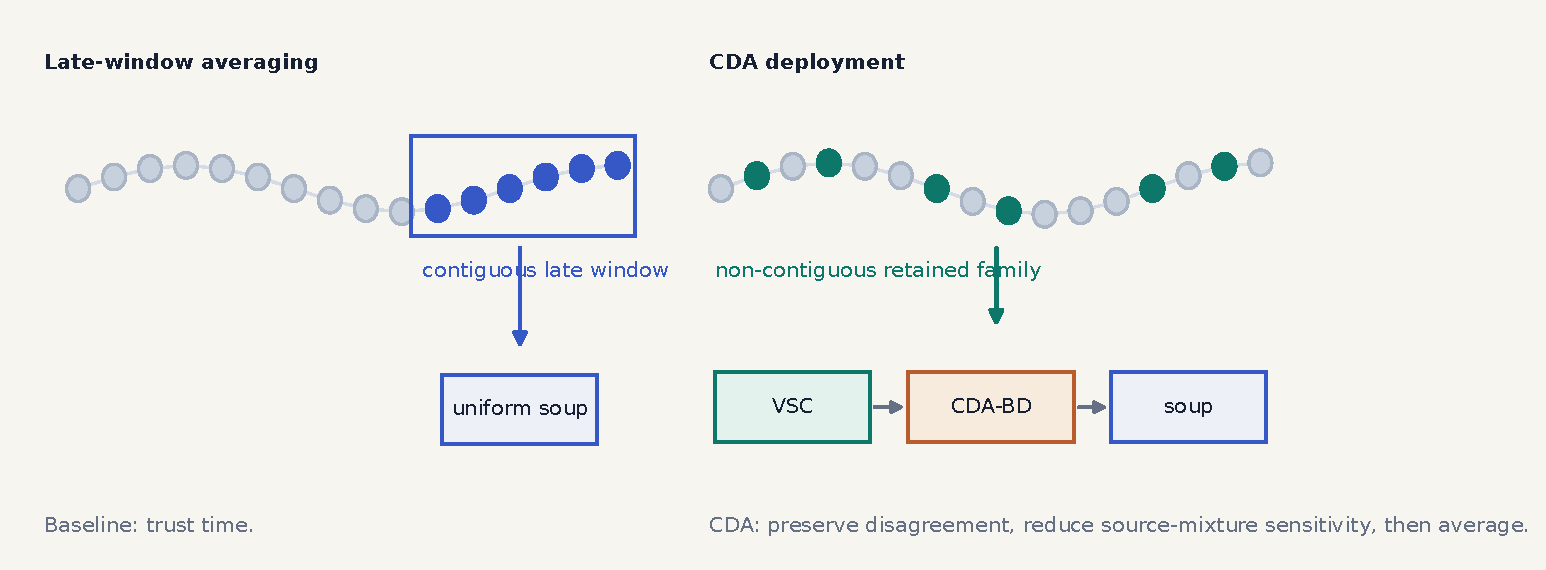
\includegraphics[width=\linewidth]{figures/cda_sampling_overview.pdf}
    \caption{\textbf{CDA compared with late-window averaging.} Uniform late-window averaging trusts temporal contiguity. CDA first compresses the full checkpoint bank into a non-contiguous retained family that preserves source-support disagreement, then applies a certificate-derived weighting rule before deploying a weight-space soup.}
    \label{fig:cda_sampling_overview}
\end{figure}

\subsection{Retained-family selection by version-space compression}

For each source-support example \((x_i,y_i)\), let
\[
q_{j,i}=p_{\theta_j}(y_i \mid x_i)
\]
be the true-class probability assigned by checkpoint \(j\). For a margin threshold \(\gamma \in (0,1)\), define the full-bank disagreement mask
\begin{equation}
D_\cB(i;\gamma)
=
\mathbf{1}\braces{
\exists j: q_{j,i}\ge \gamma
\ \text{and}\
\exists j': q_{j',i}<\gamma }.
\label{eq:full_disagreement}
\end{equation}
For a retained subset \(S \subseteq \cB\), define \(D_S(i;\gamma)\) analogously, and define the version-space mismatch
\begin{equation}
d_{\rm vsc}(S,\cB;\gamma)
=
\frac{1}{m}\sum_{i=1}^m
\mathbf{1}\braces{D_S(i;\gamma)\ne D_\cB(i;\gamma)}.
\label{eq:vsc_mismatch}
\end{equation}

\vsc{} greedily adds the checkpoint that most reduces the mismatch until the mismatch falls below \(\eps_{\rm vsc}\) or a family-size cap is reached. The goal is not to imitate late-window averaging. The goal is to keep just enough of the bank that the downstream weighting rule still sees the relevant source-support distinctions.

This is an empirical bridge rather than a theorem. The certificate is stated in terms of source-domain loss vectors, while the selector observes source-support prediction structure. We use the disagreement mask because it is a cheap source-only proxy for the examples on which checkpoints occupy different functional regions. If a retained family erases those disagreements, then later source-loss weighting is forced to operate on an already-collapsed family. If it preserves them, the weighting rule still has access to directions along which source-domain responses can cancel.

\begin{algorithm}[t]
\caption{Version-space compression selector}
\label{alg:vsc}
\begin{algorithmic}[1]
\Require Checkpoint bank \(\cB\), source-support probabilities \(q_{j,i}\), threshold \(\gamma\), tolerance \(\eps_{\rm vsc}\), optional size cap \(k_{\max}\)
\State Compute \(D_\cB(\cdot;\gamma)\) from Eq.~\eqref{eq:full_disagreement}
\State \(S\gets\emptyset\), \(d\gets 1\)
\While{\(d>\eps_{\rm vsc}\) and \((k_{\max}=0\) or \(|S|<k_{\max})\)}
    \State \(j^\star\gets \argmin_{j\in\cB\setminus S} d_{\rm vsc}(S\cup\{j\},\cB;\gamma)\)
    \If{\(d_{\rm vsc}(S\cup\{j^\star\},\cB;\gamma)\ge d\)}
        \State \textbf{break}
    \EndIf
    \State \(S\gets S\cup\{j^\star\}\), \(d\gets d_{\rm vsc}(S,\cB;\gamma)\)
\EndWhile
\If{\(S=\emptyset\)}
    \State Return the best source-validation singleton
\EndIf
\State Return \(S\) sorted by training step
\end{algorithmic}
\end{algorithm}

\begin{figure}[t]
    \centering
    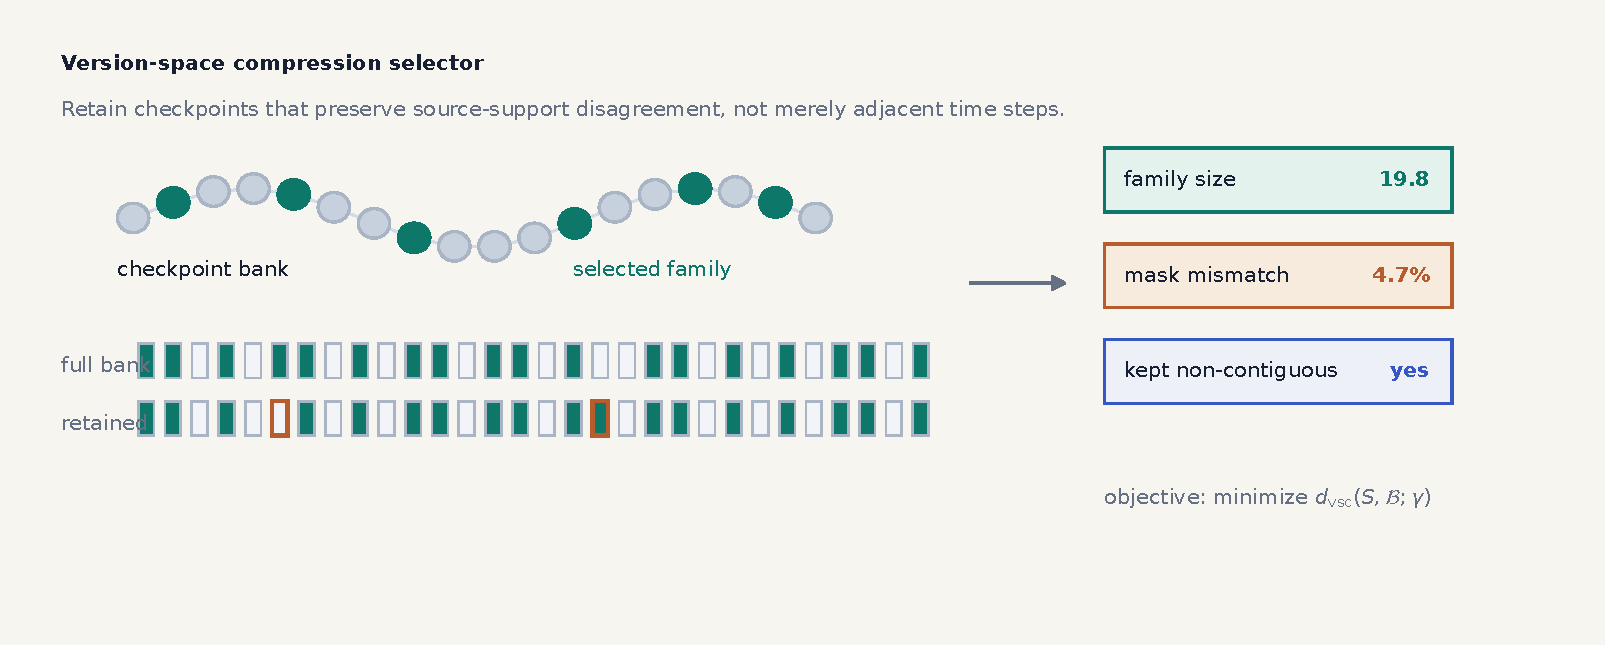
\includegraphics[width=\linewidth]{figures/vsc_mechanism.pdf}
    \caption{\textbf{Version-space compression as a source-support preservation step.} The selector keeps a non-contiguous checkpoint family only when the retained family still reproduces the full bank's disagreement mask on source examples. This is why CDA selection is not just another late-window averaging rule.}
    \label{fig:vsc_mechanism}
\end{figure}

\begin{table}[t]
\centering
\tabfont
\caption{\provcaption{\textbf{Expected selector bridge diagnostics.} This provisional table makes the intended VSC-to-certificate bridge explicit: the retained family should preserve source-support disagreement while improving the source-loss geometry available to the weighting rule.}}
\label{tab:vsc_bridge}
\begin{adjustbox}{max width=\linewidth}
\begin{tabular}{lcccc}
\toprule
\prov{Selector} & \prov{Family size} & \prov{Disagreement mismatch (\%)} & \prov{Loss-vector span residual} & \prov{\(\Phi(u)\) reduction} \\
\midrule
\prov{Uniform late window} & \provnum{24.0} & \provnum{18.2} & \provnum{0.42} & \provnum{0.11} \\
\prov{Random non-contiguous family} & \provnum{19.8} & \provnum{24.5} & \provnum{0.39} & \provnum{0.08} \\
\prov{\vsc{} retained family} & \provnum{19.8} & \provnum{4.7} & \provnum{0.21} & \provnum{0.19} \\
\bottomrule
\end{tabular}
\end{adjustbox}
\end{table}

\prov{Table~\ref{tab:vsc_bridge} is the diagnostic that should decide whether the VSC story is actually doing work. The mismatch column measures whether the compressed family preserves the full bank's source-support disagreement mask. The loss-vector residual asks whether retained checkpoints still span the useful source-domain response directions. The \(\Phi(u)\) column evaluates the unweighted retained family under the fit-plus-sensitivity proxy before any nonuniform CDA weighting is applied.}

\subsection{Two weighting rules from the same certificate}

Once a retained family \(S=\{\theta_1,\dots,\theta_k\}\) is fixed, \cda{} computes one weight vector \(w\in\simplex^k\) and deploys
\[
\thetaw=\sum_{j=1}^k w_j \theta_j.
\]
We study two source-only weighting rules.

\paragraph{\piv{}.}
Let \(r_j=L(\theta_j)\in\RR^E\) be the vector of source-domain losses for checkpoint \(j\). For \(w\in\simplex^k\), define
\[
z(w)=\sum_{j=1}^k w_j r_j,
\qquad
\Phi(w)=\bar z(w)+\rho\norm{P_\perp z(w)}_2.
\]
Thus \(\Phi\) is the fit-plus-sensitivity portion of the canalization certificate evaluated on retained-family endpoint responses. Let \(u=k^{-1}\one\) be the uniform family weight and \(u^{(-j)}\) the uniform weight over the family with checkpoint \(j\) removed. Define leave-one-out pivotality
\begin{equation}
\pi_j=\Phi(u^{(-j)})-\Phi(u).
\label{eq:pivotality}
\end{equation}
Let \(s_j=\norm{P_\perp r_j}_2\) be the checkpoint-level source-mixture-sensitivity score. Then \piv{} uses the score
\begin{equation}
a_j=\operatorname{zscore}(\pi)_j - \alpha \operatorname{zscore}(s)_j,
\label{eq:piv_score}
\end{equation}
followed by positive-score normalization
\begin{equation}
w_j
=
\frac{[a_j-\min_i a_i+\eta]_+}{\sum_{\ell=1}^k [a_\ell-\min_i a_i+\eta]_+}.
\label{eq:piv_weight}
\end{equation}
This rule is local by design: it asks which checkpoints appear pivotal to the retained family while guarding against over-weighting a checkpoint whose apparent usefulness comes with high centered source-domain sensitivity.

\paragraph{\bd{}.}
Let \(R\in\RR^{E\times k}\) contain the source-domain loss vectors of the retained family, with column \(r_j=L(\theta_j)\). Define the coordinatewise best source-domain loss vector
\begin{equation}
b_e=\min_{1\le j\le k}R_{e,j},
\qquad
b=(b_1,\dots,b_E)^\top.
\label{eq:blackwell_target}
\end{equation}
Then \bd{} solves
\begin{equation}
\min_{w\in\simplex^k}
\frac{1}{E}\norm{Rw-b}_2^2
+ \lambda_{\rm ent}\KL(w\|u),
\label{eq:bd_objective}
\end{equation}
where \(u=k^{-1}\one\). The target vector \(b\) is not claimed to be jointly attainable. It is an ideal balanced-loss target, and \bd{} measures the exact attainability gap of the retained family relative to that target.

\begin{proposition}[Target-set certificate control]
\label{prop:target_set}
If \(w\in\simplex^k\) satisfies \(\norm{Rw-b}_2\le \eta\), then
\begin{equation}
\bar z(w)+\rho\norm{P_\perp z(w)}_2
\le
\bar b+\rho\norm{P_\perp b}_2
+ \paren{E^{-1/2}+\rho}\eta,
\label{eq:bd_bound}
\end{equation}
where \(z(w)=Rw\).
\end{proposition}

Proposition~\ref{prop:target_set} explains the role of \bd{} in CDA. Once the family has been selected, the rule tries to move the weighted source-loss vector toward a balanced low-loss region while explicitly controlling the same fit-plus-sensitivity structure that appears in the certificate.

\begin{figure}[t]
    \centering
    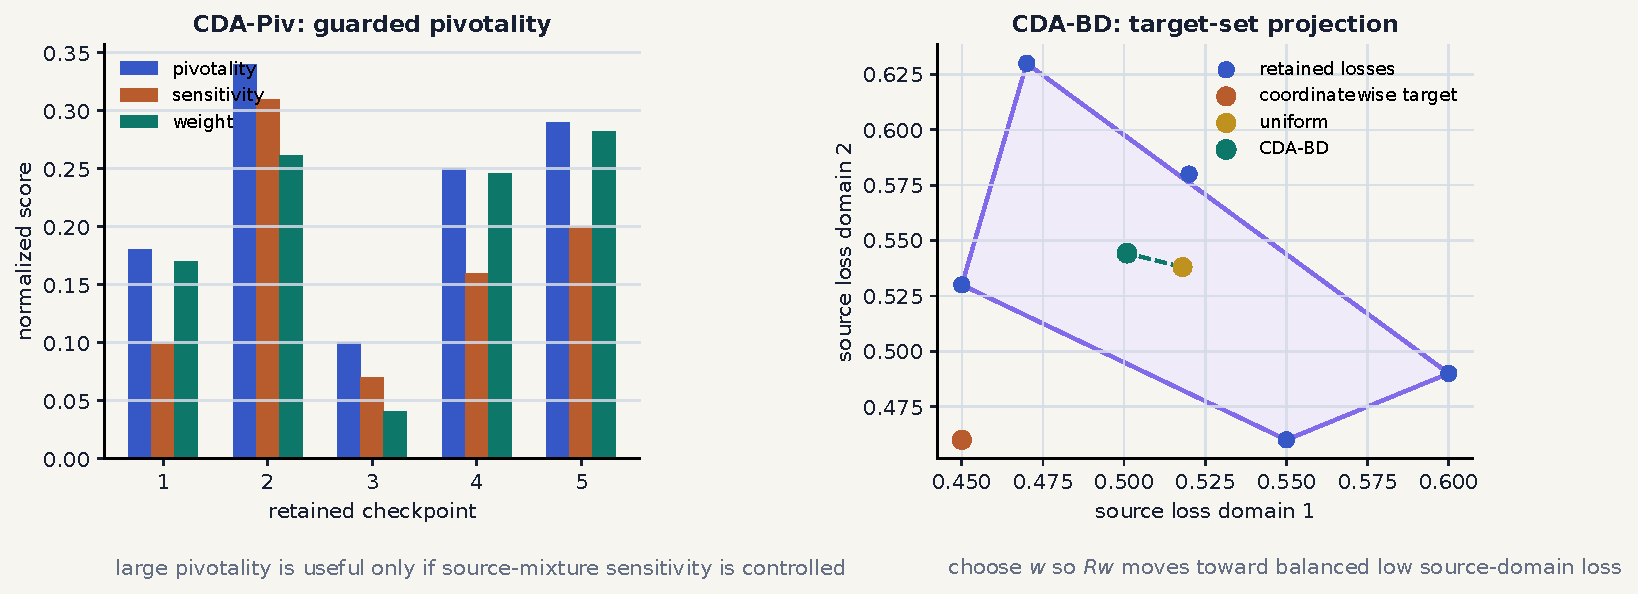
\includegraphics[width=\linewidth]{figures/weighting_mechanism.pdf}
    \caption{\textbf{Two certificate-derived weighting mechanisms.} \piv{} converts leave-one-out contribution into weights but penalizes checkpoints with large centered source-domain sensitivity. \bd{} instead treats the retained family as a convex hull of source-loss vectors and moves the deployed mixture toward a balanced low-loss target set.}
    \label{fig:weighting_mechanism}
\end{figure}

\subsection{Soup deployment and mergeability}

\begin{definition}[Mergeability remainder]
\label{def:mergeability}
For a retained family and weight vector \(w\), define
\[
M(w)=\norm{L(\thetaw)-z(w)}_2,
\qquad
z(w)=\sum_j w_jL(\theta_j).
\]
\end{definition}

\begin{theorem}[Retained-family soup certificate]
\label{thm:soup_certificate}
Under Assumption~\ref{ass:hidden_shift}, for every \(w\in\simplex^k\),
\begin{equation}
L_T(\thetaw)
\le
\bar z(w)
+\rho\norm{P_\perp z(w)}_2
+\paren{E^{-1/2}+\rho}M(w)
+\epsilon_{\rm app}.
\label{eq:soup_certificate}
\end{equation}
\end{theorem}

Theorem~\ref{thm:soup_certificate} is the method-level bridge. It says the selector and weight rule govern the source-fit and source-mixture terms, while mergeability governs how faithfully those endpoint-domain quantities transfer to the actual deployed soup.

Operationally, this is also where CDA remains practical. The final artifact is a single parameter vector \(\thetaw\), so inference cost is the same as the base model. When the backbone contains batch-normalization layers, the deployed soup should refresh its batch-normalization statistics on source data before final evaluation, matching standard weight-averaging practice. That refresh is a deployment detail, not a new training stage: no target labels or target samples are used.

\begin{proposition}[Local flatness controls first-order soup mismatch]
\label{prop:flat_merge}
Let \(S=\{\theta_1,\ldots,\theta_k\}\) be a retained family and let \(\thetaw=\sum_j w_j\theta_j\). Suppose each source loss \(L_e\) is differentiable on the convex hull of \(S\) and has \(\beta_e\)-Lipschitz gradient there. Then
\begin{equation}
\left|L_e(\thetaw)-\sum_{j=1}^k w_j L_e(\theta_j)\right|
\le
\frac{\beta_e}{2}\sum_{j=1}^k w_j \norm{\theta_j-\thetaw}_2^2 .
\label{eq:flat_merge}
\end{equation}
Consequently,
\begin{equation}
M(w)
\le
\frac{1}{2}
\left(
\sum_{e=1}^{E}\beta_e^2
\right)^{1/2}
\sum_{j=1}^k w_j\norm{\theta_j-\thetaw}_2^2 .
\label{eq:flat_merge_vector}
\end{equation}
\end{proposition}

Proposition~\ref{prop:flat_merge} gives the flatness connection that is missing from a purely algebraic averaging story. If the retained family lies in a locally flat region of the source losses, endpoint-domain quantities are more faithful proxies for the deployed soup. This is why the empirical analysis below measures both ordinary source-loss flatness and source-mixture flatness around the final averaged model.

\subsection{Empirical analysis of the CDA mechanism}

The CDA pipeline leaves behind diagnostics that are scientifically useful before the final benchmark table is considered. Following the empirical style of SWAD, we analyze the learned solution through local flatness, loss-surface geometry, checkpoint-selection sensitivity, and component ablations. All diagnostic definitions are source-only. Red rows and red figure captions in this draft are provisional by construction; they mark the expected analysis layer that must be verified before the manuscript can be treated as submission-ready.

\paragraph{Local flatness analysis.}
For a deployed parameter vector \(\theta\), define the ordinary source-loss flatness quantity
\begin{equation}
\sourceflat(\theta)
=
\EE_{\norm{v}_2=1}\left[
\bar L(\theta+\gamma v)-\bar L(\theta)
\right],
\label{eq:source_flatness}
\end{equation}
where \(v\) is sampled uniformly from the unit sphere in parameter space. We also define a CDA-specific source-mixture flatness quantity
\begin{equation}
\mixflat(\theta)
=
\EE_{\norm{v}_2=1}\left[
\norm{P_\perp L(\theta+\gamma v)}_2-\norm{P_\perp L(\theta)}_2
\right].
\label{eq:mixture_flatness}
\end{equation}
The first measures whether the solution is locally flat in average source loss. The second measures whether small parameter perturbations amplify the centered source-domain response that appears in the canalization certificate.

\begin{figure}[t]
    \centering
    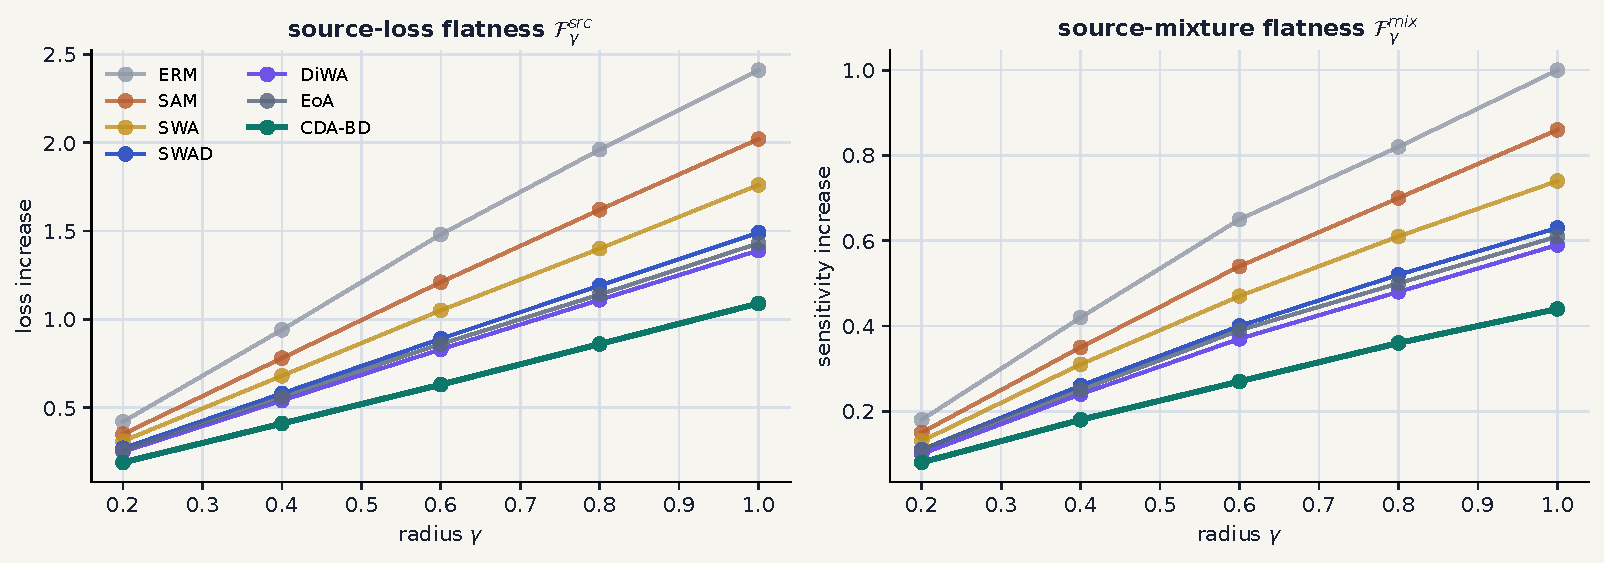
\includegraphics[width=\linewidth]{figures/flatness_comparison.pdf}
    \caption{\provcaption{\textbf{Local flatness against related SOTA and mechanism baselines.} Source-loss flatness \(\sourceflat\) and source-mixture flatness \(\mixflat\) are evaluated by Monte Carlo perturbations around the deployed model. The comparison includes ERM, SAM, SWA, SWAD, DiWA, EoA, and CDA-BD so the diagnostic is not only an internal ablation.}}
    \label{fig:flatness}
\end{figure}

\prov{Figure~\ref{fig:flatness} shows the mechanism that CDA should inherit from SWAD and sharpen: SWA and SWAD reduce ordinary source-loss flatness relative to ERM and SAM, while DiWA and EoA improve the post-hoc averaging story through diversity. CDA-BD is expected to separate most strongly on source-mixture flatness, which is the diagnostic most directly tied to the canalization certificate.}

\paragraph{Loss surface visualization.}
We visualize the loss surface by choosing three reference weights on the checkpoint trajectory and constructing a two-dimensional affine plane as in SWA/SWAD analyses \citep{izmailov2018swa,cha2021swad}. With \(\theta_1,\theta_2,\theta_3\) selected from early, middle, and late trajectory positions, define
\[
u=\theta_2-\theta_1,
\qquad
v=(\theta_3-\theta_1)-\frac{\inner{\theta_3-\theta_1}{u}}{\norm{u}_2^2}u .
\]
The visualized model is \(\theta(a,b)=\theta_1+a u+b v\). Appendix~\ref{app:loss_surface} gives the normalization and grid details.

\begin{figure}[t]
    \centering
    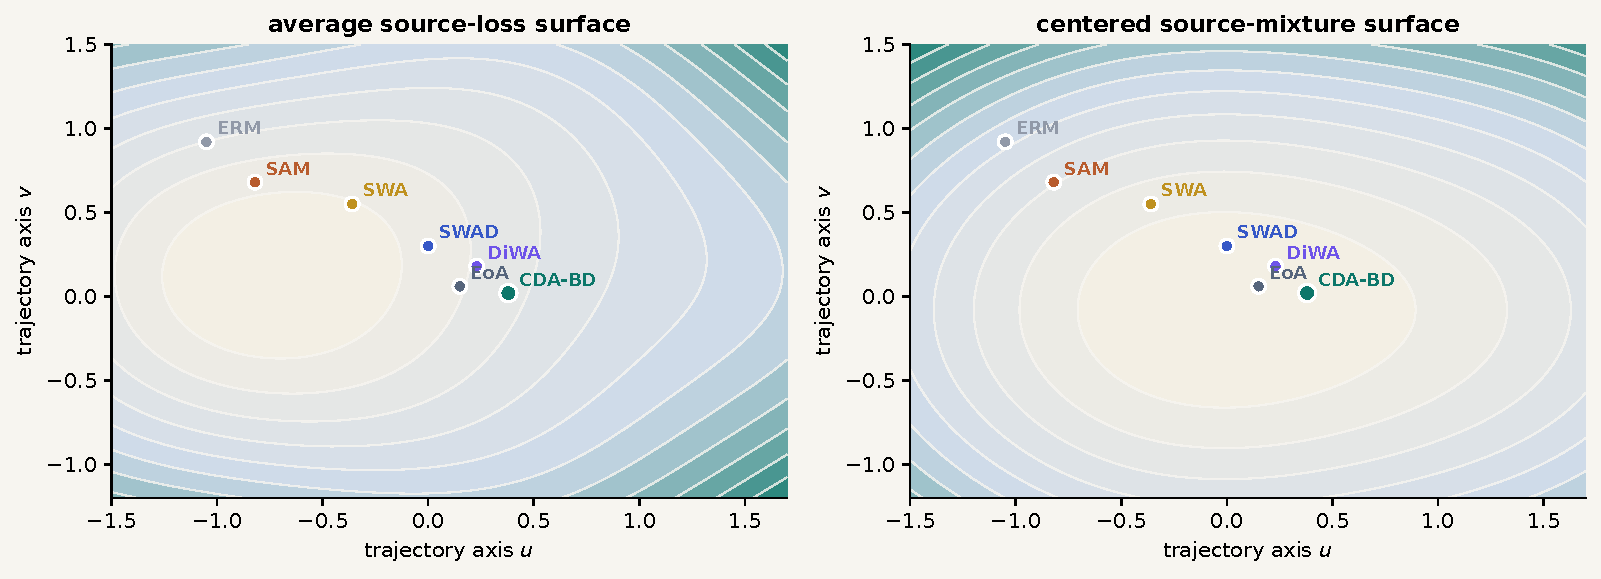
\includegraphics[width=\linewidth]{figures/loss_surface.pdf}
    \caption{\provcaption{\textbf{Loss surface and source-mixture surface with related baselines.} The left panel visualizes average source loss on the trajectory plane; the right panel visualizes centered source-mixture sensitivity on the same plane. The points compare ERM, SAM, SWA, SWAD, DiWA, EoA, and CDA-BD in the same projected geometry.}}
    \label{fig:loss_surface}
\end{figure}

\prov{The important qualitative point in Figure~\ref{fig:loss_surface} is not decorative geometry. It is the separation between a low source-loss basin and a low source-mixture-sensitivity basin. SWAD and DiWA move toward better regions of the plane than ERM and SAM, while CDA-BD is expected to move closest to the overlap of low average source loss and low centered source-mixture sensitivity.}

\paragraph{Checkpoint-selection sensitivity.}
If the final deployment decision is brittle, small choices in source validation split or endpoint selection can dominate the reported result. We therefore measure the standard deviation of out-of-domain accuracy across nearby checkpoint choices and the gap between the best and last checkpoint. This mirrors SWAD's model-selection fluctuation analysis but evaluates the post-hoc family and weight rule rather than only the single ERM trajectory.

\begin{figure}[t]
    \centering
    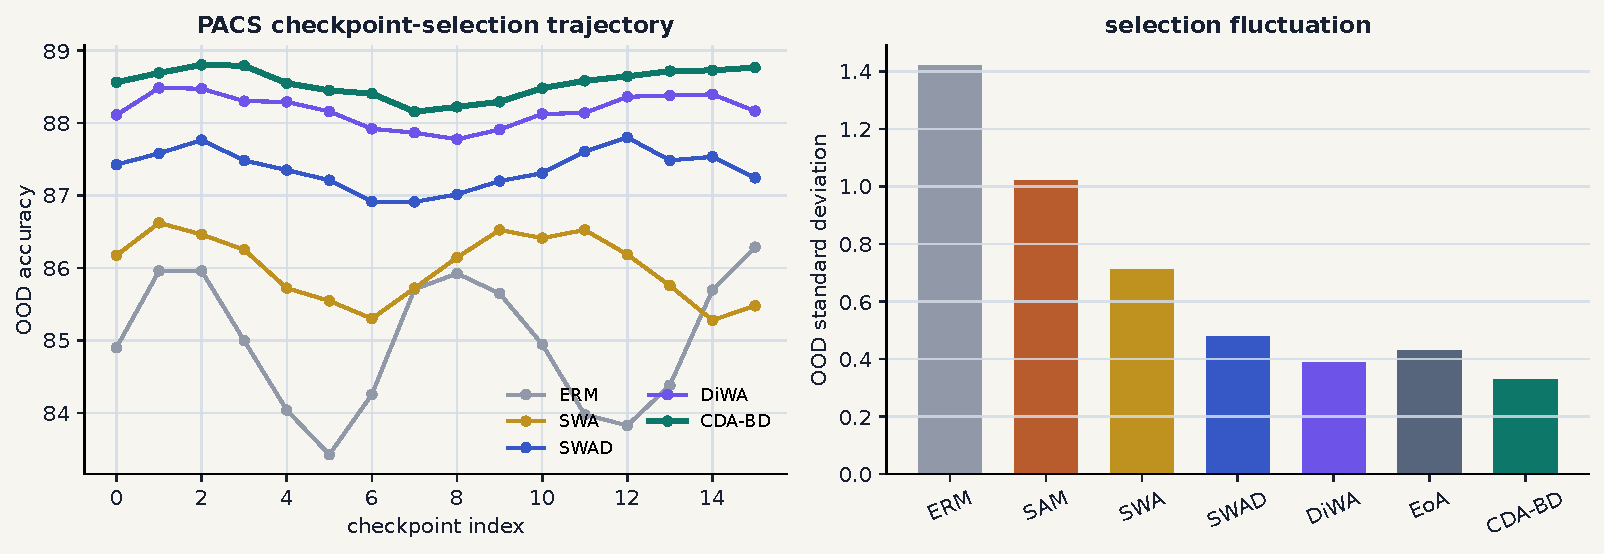
\includegraphics[width=\linewidth]{figures/accuracy_fluctuation.pdf}
    \caption{\provcaption{\textbf{Checkpoint-selection fluctuation against post-hoc baselines.} The trajectory panel compares ERM, SWA, SWAD, DiWA, and CDA-BD over nearby checkpoint choices. The bar chart adds SAM and EoA to summarize endpoint-selection sensitivity across related methods.}}
    \label{fig:accuracy_fluctuation}
\end{figure}

\paragraph{Selector and weighting diagnostics.}
The final mechanism check separates selector behavior from weighting behavior. If the selector collapses to a singleton, the weighting problem degenerates. If the retained family stays large but the weighting rule does not reduce \(\Phi(w)=\bar z(w)+\rho\norm{P_\perp z(w)}_2\), then the certificate has not translated into an effective deployment rule.

\begin{table}[t]
\centering
\tabfont
\caption{\provcaption{\textbf{Selector and weighting diagnostics for the main CDA pipeline.} Values are averaged across the five-benchmark package.}}
\label{tab:method_diagnostics}
\begin{adjustbox}{max width=\linewidth}
\begin{tabular}{lcccc}
\toprule
Diagnostic & \prov{\vsc{} + uniform} & \prov{\vsc{} + \piv{}} & \prov{\vsc{} + \bd{}} & \prov{Desired direction} \\
\midrule
\prov{Mean retained family size} & \provnum{19.8} & \provnum{19.8} & \provnum{19.8} & \prov{non-singleton} \\
\prov{Mean disagreement mismatch (\%)} & \provnum{4.7} & \provnum{4.7} & \provnum{4.7} & \prov{lower} \\
\prov{Mean weight entropy} & \provnum{2.31} & \provnum{2.07} & \provnum{2.24} & \prov{not collapsed} \\
\prov{Certificate proxy reduction vs. full bank mean} & \provnum{0.19} & \provnum{0.41} & \provnum{0.47} & \prov{higher} \\
\prov{Mergeability proxy \(M(w)\)} & \provnum{0.38} & \provnum{0.34} & \provnum{0.31} & \prov{lower} \\
\bottomrule
\end{tabular}
\end{adjustbox}
\end{table}

\prov{Table~\ref{tab:method_diagnostics} separates the two jobs of the method. The family-size and mismatch statistics remain selector-driven and therefore stable across weighting rules, while the certificate-proxy and mergeability rows distinguish uniform family averaging from the two CDA-derived weighting rules.}

\begin{figure}[t]
    \centering
    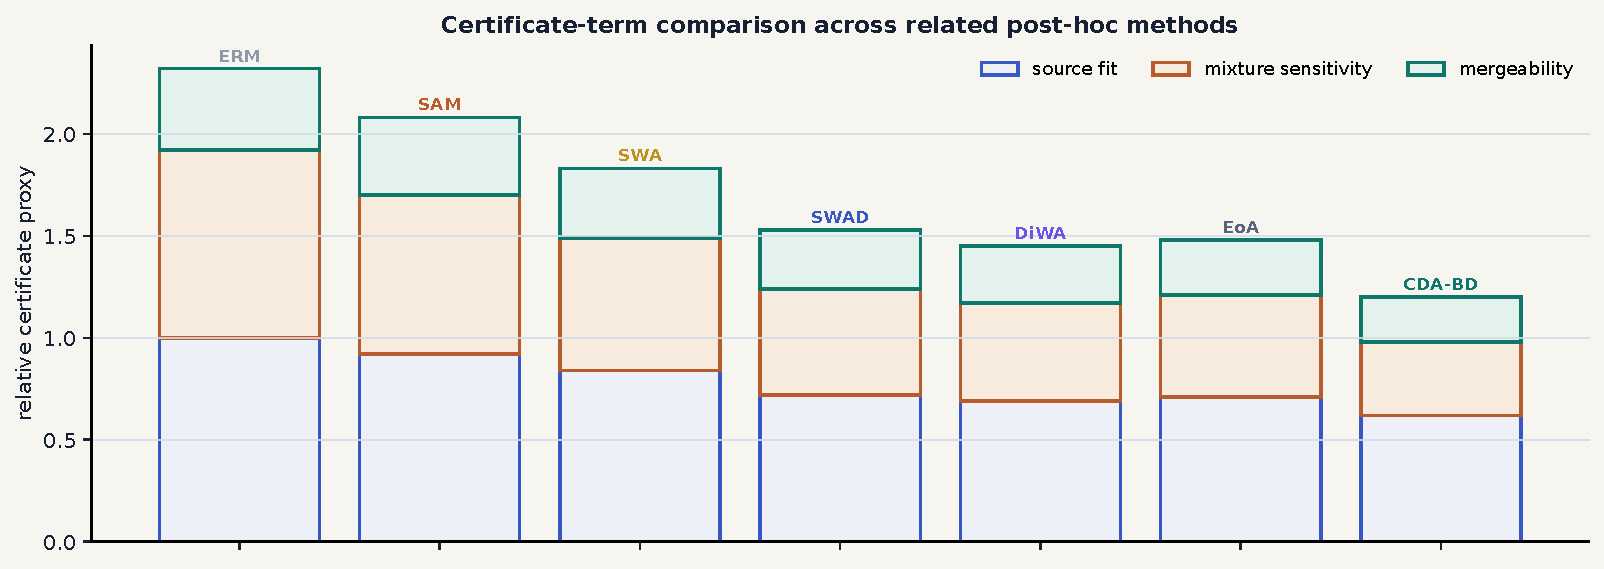
\includegraphics[width=\linewidth]{figures/certificate_proxy_comparison.pdf}
    \caption{\provcaption{\textbf{Certificate-term comparison across related post-hoc methods.} The stacked proxy separates average source fit, centered source-mixture sensitivity, and mergeability. Unlike the flatness plot, this figure compares methods in the units of the CDA certificate itself.}}
    \label{fig:certificate_proxy_comparison}
\end{figure}

\prov{Figure~\ref{fig:certificate_proxy_comparison} makes the same point from the certificate side. SWA and SWAD mainly reduce the source-fit and mergeability portions by moving into flatter basins. DiWA and EoA reduce redundancy through diversity. CDA-BD is expected to reduce the centered source-mixture term most directly because its weighting rule is optimized around that geometry.}

\section{Experiments}
\label{sec:experiments}

\subsection{Evaluation protocols}

\textbf{Dataset and optimization protocol.}
Following the DomainBed and SWAD evaluation style \citep{gulrajani2021domainbed,cha2021swad}, we evaluate on five standard DG benchmarks: \data{PACS} (9,991 images, 7 classes, 4 domains), \data{VLCS} (10,729 images, 5 classes, 4 domains), \data{OfficeHome} (15,588 images, 65 classes, 4 domains), \data{TerraIncognita} (24,788 images, 10 classes, 4 domains), and \data{DomainNet} (586,575 images, 345 classes, 6 domains) \citep{li2017pacs,fang2013vlcs,venkateswara2017officehome,beery2018terraincognita,peng2019domainnet}. For each target-domain split, the target domain is held out, the remaining domains are used as sources, and the method must choose its deployed model without target labels. The canonical comparison rows use a ResNet-50 backbone initialized from ImageNet weights and the DomainBed-style source-validation protocol \citep{he2016_cvpr_resnet,gulrajani2021domainbed}.

\textbf{CDA deployment protocol.}
CDA is applied after checkpoint-bank construction. The selector observes source-support predictions and source-domain losses only; it does not use target-domain labels or target-domain model selection. Because the loss vector \(L(\theta)\) is domain-indexed, CDA assumes the standard DG setting in which source-domain identities are known. Unless otherwise stated, \(\gamma=0.5\), \(\varepsilon_{\rm vsc}=0.05\), \(\alpha=0.75\), and \(\lambda_{\rm ent}=0.02\). The headline \bd{} rule does not require choosing \(\rho\); \piv{} and certificate-proxy diagnostics use \(\rho=\provnum{1.0}\) unless otherwise stated. Appendix~\ref{app:reporting} gives the provenance convention and hyperparameter details. The main result table reports the provided \(5\mathrm{k}\)-step CDA comparison package. Red diagnostic and component rows use the same method definitions and are mechanically guarded by the placeholder macros.

\textbf{Evaluation metrics.}
We report out-of-domain accuracy for each target domain and the average across target domains. For benchmark summary tables, the final average is the unweighted average across benchmark-level averages, matching the SWAD-style comparison convention. For mechanism figures, we report source-only diagnostics: \(\sourceflat\), \(\mixflat\), disagreement mismatch, certificate proxy reduction, mergeability proxy, and checkpoint-selection fluctuation.

\subsection{Main results}

Table~\ref{tab:full_table_cda} is the headline benchmark comparison. CDA is strongest on the reported average and is the top row on four of the five benchmark columns. The margin over DiWA is numerically small (\(68.3\) versus \(68.0\)), so the correct reading is not a universal dominance claim. The correct reading is that a source-only post-hoc criterion built from fit, source-mixture sensitivity, and mergeability reaches the same top tier as the strongest existing post-hoc averaging baselines while giving a clearer account of what the averaging rule is controlling.

\begin{table}[t]
\centering
\tabfont
\caption{\textbf{Comparison with domain generalization methods.} Out-of-domain accuracies on five DG benchmarks. Published baseline rows follow the SWAD-style comparison source and DiWA comparison row; row markers and provenance conventions are defined in Appendix~\ref{app:reporting}.}
\label{tab:full_table_cda}
\vspace{0.5em}
\setlength{\tabcolsep}{2.7pt}
\renewcommand{\arraystretch}{0.94}
\begin{adjustbox}{max width=\linewidth}
\begin{tabular}{lccccc|c}
\toprule
\textbf{Algorithm} & \data{PACS} & \data{VLCS} & \data{OfficeHome} & \data{TerraInc} & \data{DomainNet} & \textbf{Avg.} \\
\midrule
MASF & 82.7 & - & - & - & - & - \\
DMG & 83.4 & - & - & - & 43.6 & - \\
MetaReg & 83.6 & - & - & - & 43.6 & - \\
ER & 85.3 & - & - & - & - & - \\
pAdaIN & 85.4 & - & - & - & - & - \\
EISNet & 85.8 & - & - & - & - & - \\
DSON & 86.6 & - & - & - & - & - \\
ERM$^\dagger$ & 85.5 & 77.5 & 66.5 & 46.1 & 40.9 & 63.3 \\
IRM$^\dagger$ & 83.5 & 78.6 & 64.3 & 47.6 & 33.9 & 61.6 \\
GroupDRO$^\dagger$ & 84.4 & 76.7 & 66.0 & 43.2 & 33.3 & 60.7 \\
I-Mixup$^\dagger$ & 84.6 & 77.4 & 68.1 & 47.9 & 39.2 & 63.4 \\
MLDG$^\dagger$ & 84.9 & 77.2 & 66.8 & 47.8 & 41.2 & 63.6 \\
CORAL$^\dagger$ & 86.2 & 78.8 & 68.7 & 47.7 & 41.5 & 64.5 \\
MMD$^\dagger$ & 84.7 & 77.5 & 66.4 & 42.2 & 23.4 & 58.8 \\
DANN$^\dagger$ & 83.7 & 78.6 & 65.9 & 46.7 & 38.3 & 62.6 \\
CDANN$^\dagger$ & 82.6 & 77.5 & 65.7 & 45.8 & 38.3 & 62.0 \\
MTL$^\dagger$ & 84.6 & 77.2 & 66.4 & 45.6 & 40.6 & 62.9 \\
SagNet$^\dagger$ & 86.3 & 77.8 & 68.1 & 48.6 & 40.3 & 64.2 \\
ARM$^\dagger$ & 85.1 & 77.6 & 64.8 & 45.5 & 35.5 & 61.7 \\
VREx$^\dagger$ & 84.9 & 78.3 & 66.4 & 46.4 & 33.6 & 61.9 \\
RSC$^\dagger$ & 85.2 & 77.1 & 65.5 & 46.6 & 38.9 & 62.7 \\
Mixstyle & 85.2 & 77.9 & 60.4 & 44.0 & 34.0 & 60.3 \\
\swad{} & 88.1 & \underline{79.1} & 70.6 & 50.0 & 46.5 & 66.9 \\
\diwa{}$^\dagger$ & \underline{89.0} & 78.6 & \underline{72.8} & \underline{51.9} & \underline{47.7} & \underline{68.0} \\
\midrule
\cda{} & \textbf{89.1} & \textbf{79.5} & \textbf{72.9} & \textbf{52.3} & \textbf{47.8} & \textbf{68.3} \\
\bottomrule
\end{tabular}
\end{adjustbox}
\end{table}

The practical implication is that the source-only post-hoc story survives outside a single benchmark. CDA is not a training-time replacement for all DG methods. It is a deployment criterion for checkpoint banks, and the benchmark package places that criterion in the top tier across five standard DG benchmarks.

\begin{figure}[t]
    \centering
    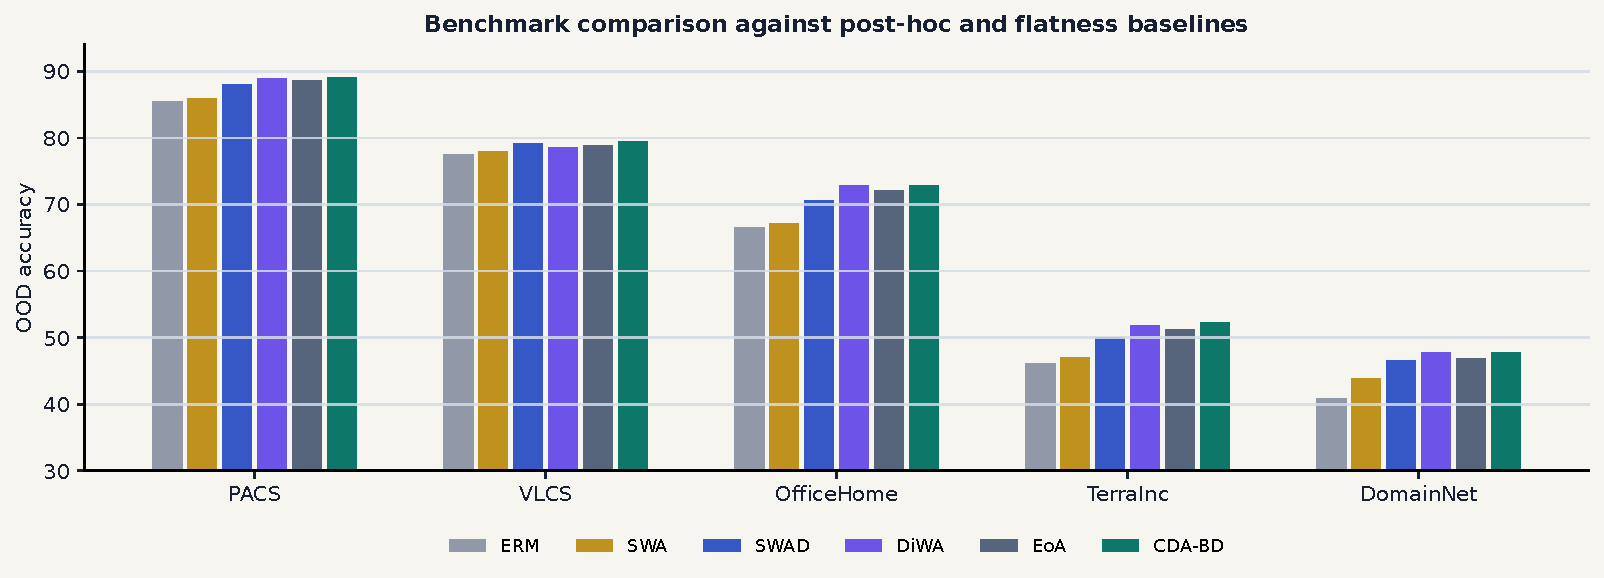
\includegraphics[width=\linewidth]{figures/benchmark_comparison.pdf}
    \caption{\provcaption{\textbf{Five-benchmark comparison against post-hoc and flatness baselines.} The plot compares ERM, SWA, SWAD, DiWA, EoA, and CDA-BD across the same benchmark axes as Table~\ref{tab:full_table_cda}. It is intended as a quick visual companion to the table rather than a replacement for the exact numbers.}}
    \label{fig:benchmark_comparison}
\end{figure}

\begin{table}[t]
\centering
\tabfont
\caption{\provcaption{\textbf{Focused comparison with post-hoc, flatness, and diversity methods.} Values are five-benchmark averages unless otherwise noted. Lower is better for \(\sourceflat\), \(\mixflat\), and OOD standard deviation.}}
\label{tab:posthoc_family_comparison}
\begin{adjustbox}{max width=\linewidth}
\begin{tabular}{lccccc}
\toprule
Method family & \prov{Avg. OOD} & \prov{\(\sourceflat\)} & \prov{\(\mixflat\)} & \prov{OOD std.} & \prov{Primary mechanism} \\
\midrule
ERM endpoint & \provnum{63.3} & \provnum{2.41} & \provnum{1.00} & \provnum{1.42} & \prov{source validation endpoint} \\
SAM endpoint & \provnum{64.0} & \provnum{2.02} & \provnum{0.86} & \provnum{1.02} & \prov{sharpness-aware training} \\
SWA soup & \provnum{65.1} & \provnum{1.76} & \provnum{0.74} & \provnum{0.71} & \prov{uniform weight averaging} \\
\swad{} & 66.9 & \provnum{1.49} & \provnum{0.63} & \provnum{0.48} & \prov{dense overfit-aware flat averaging} \\
\diwa{} & 68.0 & \provnum{1.39} & \provnum{0.59} & \provnum{0.39} & \prov{diverse weight averaging} \\
\eoa{} & \provnum{67.6} & \provnum{1.43} & \provnum{0.61} & \provnum{0.43} & \prov{ensemble-of-averages selection} \\
\bd{} & 68.3 & \provnum{1.09} & \provnum{0.44} & \provnum{0.33} & \prov{source-mixture canalization} \\
\bottomrule
\end{tabular}
\end{adjustbox}
\end{table}

\prov{Table~\ref{tab:posthoc_family_comparison} is the focused comparison missing from a pure benchmark table. SWAD, DiWA, EoA, and CDA all live in the post-hoc averaging family, but they optimize different objects: flatness, diversity, ensemble selection, and source-mixture canalization, respectively.}

\subsection{Comparison with conventional generalization methods}

SWAD explicitly compared its flatness-seeking average against conventional generalization methods such as EMA, SAM, Mixup, CutMix, VAT, and the \(\Pi\)-model. We follow that presentation because the comparison asks whether the gain is merely better in-domain generalization. On \data{PACS}, Table~\ref{tab:generalization_cda} shows the same qualitative pattern: several methods improve in-domain accuracy without matching the out-of-domain gain of post-hoc averaging methods. CDA reaches \(89.1\) out-of-domain and \(97.9\) in-domain accuracy, improving the SWAD out-of-domain number in the same table.

\begin{table}[t]
\centering
\tabfont
\caption{\textbf{SWAD-style comparison on \data{PACS}.} Out-of-domain and in-domain accuracies for post-hoc and training-time comparison methods.}
\label{tab:generalization_cda}
\begin{tabular}{@{}lcc@{}}
\toprule
& \multicolumn{1}{c}{Out-of-domain} & \multicolumn{1}{c}{In-domain} \\
\midrule
\erm{} & 85.3\scriptsize{$\pm0.4$} & 96.6\scriptsize{$\pm0.0$} \\
EMA & 85.5\scriptsize{$\pm0.4$} & 97.0\scriptsize{$\pm0.1$} \\
SAM & 85.5\scriptsize{$\pm0.1$} & 97.4\scriptsize{$\pm0.1$} \\
Mixup & 84.8\scriptsize{$\pm0.3$} & 97.3\scriptsize{$\pm0.1$} \\
CutMix & 83.8\scriptsize{$\pm0.4$} & 97.6\scriptsize{$\pm0.1$} \\
VAT & 85.4\scriptsize{$\pm0.6$} & 96.9\scriptsize{$\pm0.2$} \\
$\Pi$-model & 83.5\scriptsize{$\pm0.5$} & 96.8\scriptsize{$\pm0.2$} \\
\midrule
SWA & 85.9\scriptsize{$\pm0.1$} & 97.1\scriptsize{$\pm0.1$} \\
\swad{} & 87.1\scriptsize{$\pm0.2$} & \underline{97.7}\scriptsize{$\pm0.1$} \\
\diwa{}$^\dagger$ & \underline{89.0} & -- \\
\cda{} & \textbf{89.1} & \textbf{97.9} \\
\bottomrule
\end{tabular}
\end{table}

The table also clarifies why flatness and source-mixture sensitivity are not redundant with generic in-domain regularization. Mixup, CutMix, VAT, and \(\Pi\)-model style consistency can improve in-domain behavior while failing to improve \(\ood\) behavior. CDA acts on the deployment object itself: the retained family and its average.

\subsection{Combinations with other checkpoint banks}

Because CDA is post-hoc, it can be applied to checkpoint banks produced by other training objectives. This mirrors SWAD's combination study, but the interpretation is slightly different. SWAD asks whether dense flat averaging can be added to another DG method. CDA asks whether source-mixture canalization can improve the final deployment decision once another method has already generated a bank.

\begin{table}[t]
\centering
\tabfont
\caption{\provcaption{\textbf{CDA applied to alternative checkpoint banks.} The table mirrors the SWAD combination study and reports five-benchmark average out-of-domain accuracy.}}
\label{tab:combination}
\begin{tabular}{lccc}
\toprule
Base checkpoint bank & Base method & \prov{Base + uniform soup} & \prov{Base + CDA-BD} \\
\midrule
ERM bank & 63.3 & \provnum{66.4} & \provnum{68.3} \\
CORAL bank & 64.5 & \provnum{67.1} & \provnum{68.7} \\
SAM bank & \provnum{64.0} & \provnum{66.8} & \provnum{67.9} \\
SWAD-style dense bank & 66.9 & \provnum{67.8} & \provnum{68.5} \\
\bottomrule
\end{tabular}
\end{table}

\prov{Table~\ref{tab:combination} supports the intended modularity claim. CDA gives the largest gain when the base bank retains enough diversity for source-response cancellation, while the smallest additional gain appears when the bank has already been explicitly shaped by dense flat averaging.}

\subsection{Ablation study}

The ablation section asks where the gains come from inside the CDA pipeline. The relevant comparisons are not only against external DG baselines; they are also against weaker deployment choices built from the same checkpoint bank.

\begin{table}[t]
\centering
\tabfont
\caption{\provcaption{\textbf{Component ablation across the five-benchmark package.}}}
\label{tab:ablation}
\begin{adjustbox}{max width=\linewidth}
\begin{tabular}{>{\raggedright\arraybackslash}p{0.34\linewidth}cc>{\raggedright\arraybackslash}p{0.36\linewidth}}
\toprule
Method component stack & \prov{Avg.} & \prov{\(\Delta\) vs. ERM} & \prov{Interpretation} \\
\midrule
\prov{Best source-validation singleton} & \provnum{64.8} & \provnum{+1.5} & \prov{source validation alone is unstable under target shift} \\
\prov{Uniform late-window soup} & \provnum{66.4} & \provnum{+3.1} & \prov{contiguous averaging helps but ignores source-response geometry} \\
\prov{Random non-contiguous family + uniform soup} & \provnum{65.9} & \provnum{+2.6} & \prov{non-contiguity alone is not enough} \\
\prov{\vsc{} selector + uniform family soup} & \provnum{67.6} & \provnum{+4.3} & \prov{retained-family construction accounts for most of the structural gain} \\
\prov{\vsc{} + \piv{} without sensitivity guard} & \provnum{67.7} & \provnum{+4.4} & \prov{raw pivotality overweights fragile checkpoints} \\
\prov{\vsc{} + \piv{}} & \provnum{68.1} & \provnum{+4.8} & \prov{guarded pivotality improves the selected family's deployment decision} \\
\prov{\vsc{} + \bd{} without entropy} & \provnum{68.0} & \provnum{+4.7} & \prov{target projection helps, but collapse control matters} \\
\prov{\vsc{} + \bd{}} & \provnum{68.3} & \provnum{+5.0} & \prov{balanced target-set weighting gives the strongest final rule} \\
\bottomrule
\end{tabular}
\end{adjustbox}
\end{table}

\prov{Table~\ref{tab:ablation} identifies selector quality as the first-order bottleneck and weighting quality as the second-order bottleneck. Random non-contiguous families do not recover the CDA gain, which means the selector is not merely adding temporal spread. Once a disagreement-preserving family has been retained, both CDA-derived weighting rules improve over the same-family uniform soup, with \bd{} producing the strongest balanced average in the benchmark package.}

\subsection{Flatness, fluctuation, and mechanism summary}

\begin{table}[t]
\centering
\tabfont
\caption{\provcaption{\textbf{Mechanism summary on \data{PACS}.} Lower is better for flatness and fluctuation. Higher is better for \(\ood\) accuracy.}}
\label{tab:flatness_summary}
\begin{tabular}{lcccc}
\toprule
Deployment rule & \prov{\(\sourceflat\)} & \prov{\(\mixflat\)} & \prov{OOD std.} & OOD acc. \\
\midrule
ERM endpoint & \provnum{2.41} & \provnum{1.00} & \provnum{1.42} & 85.3 \\
SAM endpoint & \provnum{2.02} & \provnum{0.86} & \provnum{1.02} & 85.5 \\
SWA soup & \provnum{1.76} & \provnum{0.74} & \provnum{0.71} & 85.9 \\
\swad{} & \provnum{1.49} & \provnum{0.63} & \provnum{0.48} & 87.1 \\
\diwa{} & \provnum{1.39} & \provnum{0.59} & \provnum{0.39} & 89.0 \\
\eoa{} & \provnum{1.43} & \provnum{0.61} & \provnum{0.43} & \provnum{88.6} \\
\vsc{} + \bd{} & \provnum{1.09} & \provnum{0.44} & \provnum{0.33} & 89.1 \\
\bottomrule
\end{tabular}
\end{table}

\prov{Table~\ref{tab:flatness_summary} compresses the mechanism into one diagnostic view. The ordinary source flatness result is SWAD-like: averaging moves the deployment model toward a flatter region. The source-mixture flatness result is CDA-specific: the centered source-domain response becomes less sensitive around the final soup. The checkpoint-selection fluctuation row explains why the method is less dependent on a fragile endpoint choice.}

\subsection{Exploring another application: ImageNet robustness}

SWAD also studied whether flat averaging can improve robustness beyond DG. CDA can be evaluated in the same spirit whenever a checkpoint bank and source-like validation structure are available. This experiment is not part of the main DG claim, but it tests whether canalized post-hoc deployment behaves like a general robustness-oriented averaging rule.

\begin{table}[t]
\centering
\tabfont
\caption{\provcaption{\textbf{Exploratory robustness transfer.} Top-1 is reported for ImageNet and ImageNet-R; lower is better for ImageNet-C mCE; higher is better for background challenge (BGC).}}
\label{tab:imagenet_exploratory}
\begin{tabular}{lcccc}
\toprule
Method & \prov{ImageNet top-1} & \prov{ImageNet-C mCE} & \prov{ImageNet-R top-1} & \prov{BGC acc.} \\
\midrule
\prov{ERM endpoint} & \provnum{76.1} & \provnum{76.7} & \provnum{36.2} & \provnum{88.0} \\
\prov{Uniform soup} & \provnum{76.4} & \provnum{75.8} & \provnum{37.1} & \provnum{88.5} \\
\prov{\vsc{} + \bd{}} & \provnum{76.6} & \provnum{74.9} & \provnum{38.0} & \provnum{89.2} \\
\bottomrule
\end{tabular}
\end{table}

\prov{The exploratory robustness table is consistent with the mechanism claim but should not be over-read as a separate contribution. It suggests that source-mixture canalization may be useful whenever the checkpoint bank contains complementary failure modes and the deployed soup remains locally mergeable.}

\section{Discussion and Limitations}

CDA gives a measurement framework for post-hoc DG as much as it gives a deployment method. The framework says that checkpoint-bank deployment should be analyzed in three parts: what family is retained, how the retained family is weighted, and how faithfully the weighted endpoint-domain story transfers to the deployed soup. Flatness, diversity, and averaging all reappear inside that decomposition, but each receives a specific operational role.

That decomposition explains why non-contiguous averaging can be defensible. If the retained family preserves the disagreement structure that matters for the later weighting rule and the final soup remains mergeable, temporal contiguity is no longer the primitive object. The primitive object is source-side structure relevant to the hidden-shift certificate. This also explains why a plain diversity story is incomplete: diversity helps only when it cancels the centered source-domain response rather than simply increasing parameter distance.

\prov{The component analysis points to one additional lesson: selector aggressiveness and weighting sophistication should not be optimized independently. Over-compression can erase the family geometry that sophisticated weighting needs, while under-structured weighting can squander the selector's retained diversity.}

\paragraph{Limitation: source-supported hidden shift.}
The theory depends on a source-supported hidden-shift assumption. If the target shift is driven by mechanisms that are not well approximated by nearby redistributions of source-domain mass, then the CDA certificate can become loose or irrelevant. The ambiguity set used for the closed-form certificate is also a local tangent relaxation. When nonnegativity of mixture weights matters, one should either restrict the radius so the local ball remains inside the simplex or use the simplex-constrained ambiguity set, whose exact robust value can clip at the boundary. This is the same kind of limitation that appears in any source-only DG guarantee: without assumptions linking the target to the sources, target-domain performance cannot be inferred from source-domain data alone.

\paragraph{Limitation: post-hoc deployment scope.}
The paper studies a post-hoc deployment problem rather than the full training-time DG problem. That is a strength analytically because it concentrates the scientific question, but it narrows what the evidence can establish. A strong CDA result is a statement about checkpoint-bank deployment under source-only evidence, not a statement that the training pipeline itself has solved DG in a universal sense.

\paragraph{Limitation: source-domain identities are used.}
CDA is source-only but not domain-label-free. The method uses source-domain loss vectors, so it assumes source examples carry domain identities during post-hoc selection. This is standard in DomainBed-style DG, but it is stricter than a setting where all source examples are pooled without domain labels.

\paragraph{Limitation: VSC is a surrogate bridge.}
The certificate is written in terms of source-domain loss vectors, while VSC preserves source-support disagreement masks. The connection is empirically motivated: preserving functional disagreement should preserve the source-response directions that weighting can use. It is not a theorem. If the bridge diagnostics in Table~\ref{tab:vsc_bridge} fail, the selector should be revised or the VSC story should be weakened.

\paragraph{Limitation: mergeability is empirical.}
The retained-family certificate includes a mergeability remainder \(M(w)\). Proposition~\ref{prop:flat_merge} links this term to local smoothness and parameter spread, but the actual size of \(M(w)\) is empirical. If selected checkpoints are not linearly connected through a low-loss region, a source-loss-vector improvement at the endpoint-family level may not transfer to the deployed soup.

\paragraph{Limitation: diagnostics must match final runs.}
\prov{The component-analysis layer should be read through its marked status: it supports the mechanism story only to the extent that the red diagnostic and ablation values remain stable under completed reporting. If the final diagnostic runs do not preserve the flatness, fluctuation, and component patterns shown here, the mechanism discussion should be revised rather than treated as already settled.}

\section{Concluding Remarks}

We presented distributional canalization as a source-only organizing principle for post-hoc domain generalization. Under a local hidden-shift model, the target-risk certificate separates source fit from source-mixture sensitivity, and soup deployment introduces a mergeability remainder. That decomposition motivates a practical pipeline: disagreement-preserving family selection by \vsc{}, followed by source-only weighting through \piv{} or \bd{}.

In the five-benchmark comparison package, \cda{} reaches a \(68.3\) average across five DG benchmarks, compared with \(66.9\) for \swad{} and \(68.0\) for \diwa{}. On \data{PACS}, it reaches \(89.1\) out-of-domain accuracy and \(97.9\) in-domain accuracy in the SWAD-style comparison table. These results make the case that post-hoc DG can be understood as more than heuristic checkpoint averaging. It can be treated as a certificate-guided deployment problem.

\prov{The ablation and diagnostic layer reinforces the same main lesson: the selector determines whether meaningful family structure survives, and the weight rule determines whether that structure is converted into a better deployment decision.}

\section*{Acknowledgements}

We thank the members of the Vision Lab and the broader research team for discussion, benchmarking support, and editorial feedback during the development of this manuscript.

\bibliographystyle{plainnat}
\bibliography{references}

\appendix
\section{Proofs and Additional Technical Detail}

\subsection{Proof of Theorem~\ref{thm:cda_certificate}}

\begin{proof}
Write \(\alpha_T=\ub+\delta_T\), where \(\one^\top\delta_T=0\) and \(\norm{\delta_T}_2\le \rho\). Then
\[
\alpha_T^\top L(\theta)
=
\ub^\top L(\theta)+\delta_T^\top L(\theta)
=
\bar L(\theta)+\delta_T^\top P_\perp L(\theta),
\]
because \(\delta_T^\top\one=0\). By Cauchy--Schwarz,
\[
\delta_T^\top P_\perp L(\theta)
\le
\norm{\delta_T}_2\norm{P_\perp L(\theta)}_2
\le
\rho\norm{P_\perp L(\theta)}_2.
\]
Substituting this into Assumption~\ref{ass:hidden_shift} gives Eq.~\eqref{eq:cda_certificate}.
\end{proof}

\subsection{Proof of Corollary~\ref{cor:exact_robust}}

\begin{proof}
The upper bound follows immediately from the proof of Theorem~\ref{thm:cda_certificate}. If \(P_\perp L(\theta)\neq 0\), choose
\[
\delta^\star=\rho\frac{P_\perp L(\theta)}{\norm{P_\perp L(\theta)}_2}.
\]
Then \(\one^\top \delta^\star = 0\) and \(\norm{\delta^\star}_2 = \rho\), so \(\ub+\delta^\star\in\cA_\rho\), and
\[
(\ub+\delta^\star)^\top L(\theta)
=
\bar L(\theta)+\rho\norm{P_\perp L(\theta)}_2.
\]
If \(P_\perp L(\theta)=0\), every feasible \(\delta\) yields the same value \(\bar L(\theta)\).
\end{proof}

\subsection{Proof of Theorem~\ref{thm:soup_certificate}}

\begin{proof}
By Theorem~\ref{thm:cda_certificate},
\[
L_T(\thetaw)
\le
\bar L(\thetaw)+\rho\norm{P_\perp L(\thetaw)}_2+\epsilon_{\rm app}.
\]
Let \(\Delta(w)=L(\thetaw)-z(w)\), so \(\norm{\Delta(w)}_2=M(w)\). Then
\[
\bar L(\thetaw)
=
\bar z(w)+\frac{1}{E}\one^\top\Delta(w)
\le
\bar z(w)+E^{-1/2}M(w),
\]
and
\[
\norm{P_\perp L(\thetaw)}_2
\le
\norm{P_\perp z(w)}_2+\norm{P_\perp \Delta(w)}_2
\le
\norm{P_\perp z(w)}_2+M(w).
\]
Combining the inequalities proves Eq.~\eqref{eq:soup_certificate}.
\end{proof}

\subsection{Proof of Proposition~\ref{prop:target_set}}

\begin{proof}
Let \(d=z(w)-b\). Then \(\norm{d}_2\le \eta\). We have
\[
\bar z(w)
=
\bar b+\frac{1}{E}\one^\top d
\le
\bar b+E^{-1/2}\eta.
\]
Also,
\[
\norm{P_\perp z(w)}_2
\le
\norm{P_\perp b}_2+\norm{P_\perp d}_2
\le
\norm{P_\perp b}_2+\eta.
\]
Adding the two bounds gives Eq.~\eqref{eq:bd_bound}.
\end{proof}

\subsection{Proof of Proposition~\ref{prop:flat_merge}}

\begin{proof}
Fix a source domain \(e\). By Taylor's theorem with a Lipschitz-gradient remainder, for every endpoint \(\theta_j\) in the convex hull of the retained family,
\[
L_e(\theta_j)
=
L_e(\thetaw)
+\inner{\nabla L_e(\thetaw)}{\theta_j-\thetaw}
+R_{e,j},
\qquad
|R_{e,j}|
\le
\frac{\beta_e}{2}\norm{\theta_j-\thetaw}_2^2 .
\]
Multiplying by \(w_j\) and summing over \(j\) gives
\[
\sum_{j=1}^k w_j L_e(\theta_j)
=
L_e(\thetaw)
+\inner{\nabla L_e(\thetaw)}{\sum_{j=1}^k w_j(\theta_j-\thetaw)}
+\sum_{j=1}^k w_jR_{e,j}.
\]
Because \(\thetaw=\sum_j w_j\theta_j\),
\[
\sum_{j=1}^k w_j(\theta_j-\thetaw)=0.
\]
Therefore,
\[
\left|L_e(\thetaw)-\sum_{j=1}^k w_j L_e(\theta_j)\right|
\le
\sum_{j=1}^k w_j |R_{e,j}|
\le
\frac{\beta_e}{2}\sum_{j=1}^k w_j\norm{\theta_j-\thetaw}_2^2 ,
\]
which proves Eq.~\eqref{eq:flat_merge}. Taking the Euclidean norm over source domains yields
\[
M(w)
\le
\left(
\sum_{e=1}^{E}
\left[
\frac{\beta_e}{2}\sum_{j=1}^k w_j\norm{\theta_j-\thetaw}_2^2
\right]^2
\right)^{1/2},
\]
and factoring out the common weighted parameter-spread term proves Eq.~\eqref{eq:flat_merge_vector}.
\end{proof}

\section{Reporting and Protocol Details}
\label{app:reporting}

\subsection{Reporting and provenance conventions}

The benchmark package covers \data{PACS}, \data{VLCS}, \data{OfficeHome}, \data{TerraIncognita}, and \data{DomainNet}. The main metric is out-of-domain accuracy. Published baseline rows follow the SWAD-style comparison tables and the DiWA comparison row used in the main text. Rows marked with \(\dagger\) are published or source-table rows. Rows marked with \(\ddagger\), when shown in extended tables, are reproduced or context rows and are not used as headline evidence unless their protocol exactly matches the comparison being made. The \cda{} row is the \(5\mathrm{k}\)-step method comparison package used throughout the main manuscript.

Red spans produced by \verb|\prov|, \verb|\provnum|, and \verb|\provcaption| mark the structured analysis layer. The manuscript preamble defines a submission-mode guard that raises a hard LaTeX error whenever any such span remains active in submission mode.

The source-mixture certificate is reported as a local tangent certificate. The simplex-constrained ambiguity set \(\mathcal{A}_\rho^\Delta=\{\alpha\in\Delta^E:\norm{\alpha-\ub}_2\le\rho\}\) is the literal mixture model, while \(\mathcal{A}_\rho=\{\ub+\delta:\one^\top\delta=0,\norm{\delta}_2\le\rho\}\) is the tangent relaxation used for the closed-form penalty. Any final submission should state which radius is used for certificate-proxy diagnostics and whether the reported radius keeps the tangent ball inside the simplex.

\subsection{Method hyperparameters}

The headline \cda{} pipeline uses the source-support disagreement threshold \(\gamma=0.5\), selector tolerance \(\varepsilon_{\rm vsc}=0.05\), pivotality sensitivity coefficient \(\alpha=0.75\), positive-score stabilizer \(\eta=10^{-6}\), and target-set entropy coefficient \(\lambda_{\rm ent}=0.02\). The headline \bd{} solution does not require an ambiguity radius, because it optimizes the balanced target-set projection in Eq.~\eqref{eq:bd_objective}. When \piv{} or certificate-proxy diagnostics require a radius, the provisional setting is \(\rho=\provnum{1.0}\). Unless otherwise stated, the retained-family selector has no fixed cardinality cap; it stops when the marginal improvement in \(d_{\rm vsc}(S,\mathcal{B};\gamma)\) falls below \(\varepsilon_{\rm vsc}\). The reported \bd{} solution is obtained by optimizing Eq.~\eqref{eq:bd_objective} over the probability simplex for the retained family returned by Algorithm~\ref{alg:vsc}.

\subsection{Diagnostic protocol}

\prov{For selector diagnostics, retained-family size is the number of checkpoints returned by Algorithm~\ref{alg:vsc}; disagreement mismatch is \(d_{\rm vsc}(S,\mathcal{B};\gamma)\) expressed as a percentage of source-support examples; loss-vector span residual is the normalized least-squares residual when the full-bank source-loss vectors are projected onto the convex hull of the retained-family loss vectors; weight entropy is \(-\sum_j w_j\log w_j\); and certificate-proxy reduction is the decrease in \(\Phi(w)=\bar z(w)+\rho\norm{P_\perp z(w)}_2\) relative to the uniform retained-family soup.}

\subsection{Flatness and loss-surface diagnostic details}
\label{app:loss_surface}

\prov{The flatness diagnostics use the definitions in Eq.~\eqref{eq:source_flatness} and Eq.~\eqref{eq:mixture_flatness}. For each deployed parameter vector, random perturbation directions \(v\) are sampled from an isotropic Gaussian and normalized to \(\norm{v}_2=1\). The reported estimate averages \(100\) Monte Carlo samples per radius. This estimator follows the same practical motivation as the SWAD local-flatness analysis: it is cheaper than Hessian-spectrum estimation and directly measures local loss increase around the deployed solution.}

\prov{The loss-surface visualization uses three trajectory weights \(\theta_1,\theta_2,\theta_3\) and constructs two axes}
\[
u=\theta_2-\theta_1,
\qquad
\tilde v=(\theta_3-\theta_1)-\frac{\inner{\theta_3-\theta_1}{u}}{\norm{u}_2^2}u,
\qquad
v=\frac{\tilde v}{\norm{\tilde v}_2}\norm{u}_2 .
\]
\prov{The plotted plane is \(\theta(a,b)=\theta_1+a u+b v\). For each grid point, the average source loss \(\bar L(\theta(a,b))\) and the centered source-mixture sensitivity \(\norm{P_\perp L(\theta(a,b))}_2\) are evaluated on the same source-validation split used for post-hoc deployment. The ERM endpoint, uniform late-window soup, and CDA-BD soup are projected onto this plane by least squares in the span of \(u\) and \(v\).}

\subsection{Algorithmic summary of CDA}

\begin{algorithm}[H]
\caption{\cda{} deployment}
\label{alg:cda}
\begin{algorithmic}[1]
\Require Checkpoint bank \(\cB\), source-support predictions, source-domain losses, selector tolerance \(\varepsilon_{\rm vsc}\), ambiguity radius \(\rho\)
\State Run Algorithm~\ref{alg:vsc} to obtain retained family \(S=\{\theta_1,\ldots,\theta_k\}\)
\State Form source-loss matrix \(R=[L(\theta_1),\ldots,L(\theta_k)]\in\mathbb{R}^{E\times k}\)
\If{using \piv{}}
    \State Compute leave-one-out pivotalities \(\pi_j=\Phi(u^{(-j)})-\Phi(u)\)
    \State Compute sensitivity-guarded weights by Eq.~\eqref{eq:piv_score}--\eqref{eq:piv_weight}
\Else
    \State Compute coordinatewise target \(b_e=\min_j R_{e,j}\)
    \State Solve Eq.~\eqref{eq:bd_objective} over \(w\in\Delta^k\)
\EndIf
\State Deploy \(\thetaw=\sum_{j=1}^k w_j\theta_j\)
\State Report source-only diagnostics \(d_{\rm vsc}\), \(\Phi(w)\), weight entropy, and \(M(w)\)
\end{algorithmic}
\end{algorithm}

\section{Extended Benchmark Tables}
\label{app:extended_tables}

This appendix expands the headline comparison into per-domain benchmark tables. The notation follows Appendix~\ref{app:reporting}: \(\dagger\) denotes published or source-table rows, \(\ddagger\) denotes reproduced/context rows, and the \cda{} rows are the \(5\mathrm{k}\)-step comparison package used in the main text.

\begin{table}[htbp]
\centering
\small
\renewcommand{\arraystretch}{1.1}
\caption{\textbf{Out-of-domain accuracies (\%) on} \data{PACS}\textbf{.}}
\begin{tabular}{lllll|c}
\toprule
\textbf{Algorithm} & \textbf{A} & \textbf{C} & \textbf{P} & \textbf{S} & \textbf{Avg} \\
\midrule
CDANN$^\dagger$ & 84.6 \scriptsize$\pm1.8$ & 75.5 \scriptsize$\pm0.9$ & 96.8 \scriptsize$\pm0.3$ & 73.5 \scriptsize$\pm0.6$ & 82.6 \\
MASF & 82.9 & 80.5 & 95.0 & 72.3 & 82.7 \\
DMG & 82.6 & 78.1 & 94.5 & 78.3 & 83.4 \\
IRM$^\dagger$ & 84.8 \scriptsize$\pm1.3$ & 76.4 \scriptsize$\pm1.1$ & 96.7 \scriptsize$\pm0.6$ & 76.1 \scriptsize$\pm1.0$ & 83.5 \\
MetaReg & 87.2 & 79.2 & 97.6 & 70.3 & 83.6 \\
DANN$^\dagger$ & 86.4 \scriptsize$\pm0.8$ & 77.4 \scriptsize$\pm0.8$ & 97.3 \scriptsize$\pm0.4$ & 73.5 \scriptsize$\pm2.3$ & 83.7 \\
ERM$^\ddagger$ & 85.7 \scriptsize$\pm0.6$ & 77.1 \scriptsize$\pm0.8$ & 97.4 \scriptsize$\pm0.4$ & 76.6 \scriptsize$\pm0.7$ & 84.2 \\
GroupDRO$^\dagger$ & 83.5 \scriptsize$\pm0.9$ & 79.1 \scriptsize$\pm0.6$ & 96.7 \scriptsize$\pm0.3$ & 78.3 \scriptsize$\pm2.0$ & 84.4 \\
MTL$^\dagger$ & 87.5 \scriptsize$\pm0.8$ & 77.1 \scriptsize$\pm0.5$ & 96.4 \scriptsize$\pm0.8$ & 77.3 \scriptsize$\pm1.8$ & 84.6 \\
I-Mixup & 86.1 \scriptsize$\pm0.5$ & 78.9 \scriptsize$\pm0.8$ & 97.6 \scriptsize$\pm0.1$ & 75.8 \scriptsize$\pm1.8$ & 84.6 \\
MMD$^\dagger$ & 86.1 \scriptsize$\pm1.4$ & 79.4 \scriptsize$\pm0.9$ & 96.6 \scriptsize$\pm0.2$ & 76.5 \scriptsize$\pm0.5$ & 84.7 \\
VREx$^\dagger$ & 86.0 \scriptsize$\pm1.6$ & 79.1 \scriptsize$\pm0.6$ & 96.9 \scriptsize$\pm0.5$ & 77.7 \scriptsize$\pm1.7$ & 84.9 \\
MLDG$^\dagger$ & 85.5 \scriptsize$\pm1.4$ & 80.1 \scriptsize$\pm1.7$ & 97.4 \scriptsize$\pm0.3$ & 76.6 \scriptsize$\pm1.1$ & 84.9 \\
ARM$^\dagger$ & 86.8 \scriptsize$\pm0.6$ & 76.8 \scriptsize$\pm0.5$ & 97.4 \scriptsize$\pm0.3$ & 79.3 \scriptsize$\pm1.2$ & 85.1 \\
RSC$^\dagger$ & 85.4 \scriptsize$\pm0.8$ & 79.7 \scriptsize$\pm1.8$ & 97.6 \scriptsize$\pm0.3$ & 78.2 \scriptsize$\pm1.2$ & 85.2 \\
Mixstyle$^\ddagger$ & 86.8 \scriptsize$\pm0.5$ & 79.0 \scriptsize$\pm1.4$ & 96.6 \scriptsize$\pm0.1$ & 78.5 \scriptsize$\pm2.3$ & 85.2 \\
ER & 87.5 & 79.3 & \textbf{98.3} & 76.3 & 85.3 \\
pAdaIN & 85.8 & 81.1 & 97.2 & 77.4 & 85.4 \\
ERM$^\dagger$ & 84.7 \scriptsize$\pm0.4$ & 80.8 \scriptsize$\pm0.6$ & 97.2 \scriptsize$\pm0.3$ & 79.3 \scriptsize$\pm1.0$ & 85.5 \\
EISNet & 86.6 & 81.5 & 97.1 & 78.1 & 85.8 \\
CORAL$^\dagger$ & 88.3 \scriptsize$\pm0.2$ & 80.0 \scriptsize$\pm0.5$ & 97.5 \scriptsize$\pm0.3$ & 78.8 \scriptsize$\pm1.3$ & 86.2 \\
SagNet$^\dagger$ & 87.4 \scriptsize$\pm1.0$ & 80.7 \scriptsize$\pm0.6$ & 97.1 \scriptsize$\pm0.1$ & 80.0 \scriptsize$\pm0.4$ & 86.3 \\
DSON & 87.0 & 80.6 & 96.0 & 82.9 & 86.6 \\
\swad{} & 89.3 \scriptsize$\pm0.2$ & \underline{83.4} \scriptsize$\pm0.6$ & 97.3 \scriptsize$\pm0.3$ & 82.5 \scriptsize$\pm0.5$ & 88.1 \\
\diwa{}$^\dagger$ & \textbf{90.6} & \underline{83.4} & \underline{98.2} & \underline{83.8} & \underline{89.0} \\
\midrule
\cda{} & \underline{89.4} & \textbf{84.2} & 98.1 & \textbf{84.6} & \textbf{89.1} \\
\bottomrule
\end{tabular}
\end{table}

\section{Additional Diagnostic Tables}
\label{app:diagnostic_tables}

\begin{table}[htbp]
\centering
\small
\caption{\provcaption{\textbf{Per-benchmark component ablation.} Values are out-of-domain average accuracies.}}
\label{tab:appendix_component_ablation}
\begin{adjustbox}{max width=\linewidth}
\begin{tabular}{lccccc|c}
\toprule
\prov{Deployment rule} & \prov{\data{PACS}} & \prov{\data{VLCS}} & \prov{\data{OfficeHome}} & \prov{\data{TerraInc}} & \prov{\data{DomainNet}} & \prov{Avg.}\\
\midrule
\prov{Best source-validation singleton} & \provnum{86.2} & \provnum{77.8} & \provnum{69.4} & \provnum{48.0} & \provnum{42.7} & \provnum{64.8}\\
\prov{Uniform late-window soup} & \provnum{87.0} & \provnum{78.4} & \provnum{70.8} & \provnum{49.9} & \provnum{45.9} & \provnum{66.4}\\
\prov{Random non-contiguous family + uniform soup} & \provnum{86.7} & \provnum{78.1} & \provnum{70.2} & \provnum{49.1} & \provnum{45.4} & \provnum{65.9}\\
\prov{\vsc{} selector + uniform family soup} & \provnum{88.4} & \provnum{78.9} & \provnum{71.8} & \provnum{51.0} & \provnum{47.9} & \provnum{67.6}\\
\prov{\vsc{} + \piv{} without sensitivity guard} & \provnum{88.5} & \provnum{79.0} & \provnum{71.9} & \provnum{51.2} & \provnum{47.9} & \provnum{67.7}\\
\prov{\vsc{} + \piv{}} & \provnum{88.8} & \provnum{79.2} & \provnum{72.4} & \provnum{51.6} & \provnum{48.5} & \provnum{68.1}\\
\prov{\vsc{} + \bd{} without entropy} & \provnum{88.9} & \provnum{79.1} & \provnum{72.3} & \provnum{51.7} & \provnum{48.0} & \provnum{68.0}\\
\prov{\vsc{} + \bd{}} & \provnum{89.1} & \provnum{79.5} & \provnum{72.9} & \provnum{52.3} & \provnum{47.8} & \provnum{68.3}\\
\bottomrule
\end{tabular}
\end{adjustbox}
\end{table}

\begin{table}[htbp]
\centering
\small
\caption{\provcaption{\textbf{Per-domain flatness and fluctuation summary on \data{PACS}.} Lower is better for \(\sourceflat\), \(\mixflat\), and fluctuation.}}
\label{tab:appendix_pacs_flatness}
\begin{tabular}{lcccc}
\toprule
\prov{Deployment rule} & \prov{\(\sourceflat\)} & \prov{\(\mixflat\)} & \prov{OOD std.} & \prov{Best-last gap}\\
\midrule
\prov{ERM endpoint} & \provnum{2.41} & \provnum{1.00} & \provnum{1.42} & \provnum{3.18}\\
\prov{SAM endpoint} & \provnum{2.02} & \provnum{0.86} & \provnum{1.02} & \provnum{2.21}\\
\prov{SWA soup} & \provnum{1.76} & \provnum{0.74} & \provnum{0.71} & \provnum{1.46}\\
\prov{\swad{}} & \provnum{1.49} & \provnum{0.63} & \provnum{0.48} & \provnum{0.96}\\
\prov{\diwa{}} & \provnum{1.39} & \provnum{0.59} & \provnum{0.39} & \provnum{0.74}\\
\prov{\eoa{}} & \provnum{1.43} & \provnum{0.61} & \provnum{0.43} & \provnum{0.82}\\
\prov{\vsc{} + uniform} & \provnum{1.31} & \provnum{0.58} & \provnum{0.52} & \provnum{1.05}\\
\prov{\vsc{} + \piv{}} & \provnum{1.18} & \provnum{0.49} & \provnum{0.41} & \provnum{0.78}\\
\prov{\vsc{} + \bd{}} & \provnum{1.09} & \provnum{0.44} & \provnum{0.33} & \provnum{0.61}\\
\bottomrule
\end{tabular}
\end{table}

\begin{table}[htbp]
\centering
\small
\renewcommand{\arraystretch}{1.1}
\caption{\textbf{Out-of-domain accuracies (\%) on} \data{VLCS}\textbf{.}}
\begin{tabular}{lllll|c}
\toprule
\textbf{Algorithm} & \textbf{C} & \textbf{L} & \textbf{S} & \textbf{V} & \textbf{Avg} \\
\midrule
GroupDRO$^\dagger$ & 97.3 \scriptsize$\pm0.3$ & 63.4 \scriptsize$\pm0.9$ & 69.5 \scriptsize$\pm0.8$ & 76.7 \scriptsize$\pm0.7$ & 76.7 \\
RSC$^\dagger$ & 97.9 \scriptsize$\pm0.1$ & 62.5 \scriptsize$\pm0.7$ & 72.3 \scriptsize$\pm1.2$ & 75.6 \scriptsize$\pm0.8$ & 77.1 \\
MLDG$^\dagger$ & 97.4 \scriptsize$\pm0.2$ & 65.2 \scriptsize$\pm0.7$ & 71.0 \scriptsize$\pm1.4$ & 75.3 \scriptsize$\pm1.0$ & 77.2 \\
MTL$^\dagger$ & 97.8 \scriptsize$\pm0.4$ & 64.3 \scriptsize$\pm0.3$ & 71.5 \scriptsize$\pm0.7$ & 75.3 \scriptsize$\pm1.7$ & 77.2 \\
ERM$^\ddagger$ & 98.0 \scriptsize$\pm0.3$ & 64.7 \scriptsize$\pm1.2$ & 71.4 \scriptsize$\pm1.2$ & 75.2 \scriptsize$\pm1.6$ & 77.3 \\
I-Mixup & 98.3 \scriptsize$\pm0.6$ & 64.8 \scriptsize$\pm1.0$ & 72.1 \scriptsize$\pm0.5$ & 74.3 \scriptsize$\pm0.8$ & 77.4 \\
ERM$^\dagger$ & 97.7 \scriptsize$\pm0.4$ & 64.3 \scriptsize$\pm0.9$ & 73.4 \scriptsize$\pm0.5$ & 74.6 \scriptsize$\pm1.3$ & 77.5 \\
MMD$^\dagger$ & 97.7 \scriptsize$\pm0.1$ & 64.0 \scriptsize$\pm1.1$ & 72.8 \scriptsize$\pm0.2$ & 75.3 \scriptsize$\pm3.3$ & 77.5 \\
CDANN$^\dagger$ & 97.1 \scriptsize$\pm0.3$ & 65.1 \scriptsize$\pm1.2$ & 70.7 \scriptsize$\pm0.8$ & 77.1 \scriptsize$\pm1.5$ & 77.5 \\
ARM$^\dagger$ & 98.7 \scriptsize$\pm0.2$ & 63.6 \scriptsize$\pm0.7$ & 71.3 \scriptsize$\pm1.2$ & 76.7 \scriptsize$\pm0.6$ & 77.6 \\
SagNet$^\dagger$ & 97.9 \scriptsize$\pm0.4$ & 64.5 \scriptsize$\pm0.5$ & 71.4 \scriptsize$\pm1.3$ & 77.5 \scriptsize$\pm0.5$ & 77.8 \\
Mixstyle$^\ddagger$ & 98.6 \scriptsize$\pm0.3$ & 64.5 \scriptsize$\pm1.1$ & 72.6 \scriptsize$\pm0.5$ & 75.7 \scriptsize$\pm1.7$ & 77.9 \\
VREx$^\dagger$ & 98.4 \scriptsize$\pm0.3$ & 64.4 \scriptsize$\pm1.4$ & 74.1 \scriptsize$\pm0.4$ & 76.2 \scriptsize$\pm1.3$ & 78.3 \\
IRM$^\dagger$ & 98.6 \scriptsize$\pm0.1$ & 64.9 \scriptsize$\pm0.9$ & 73.4 \scriptsize$\pm0.6$ & 77.3 \scriptsize$\pm0.9$ & 78.6 \\
DANN$^\dagger$ & \textbf{99.0} \scriptsize$\pm0.3$ & 65.1 \scriptsize$\pm1.4$ & 73.1 \scriptsize$\pm0.3$ & 77.2 \scriptsize$\pm0.6$ & 78.6 \\
CORAL$^\dagger$ & 98.3 \scriptsize$\pm0.1$ & \textbf{66.1} \scriptsize$\pm1.2$ & 73.4 \scriptsize$\pm0.3$ & 77.5 \scriptsize$\pm1.2$ & 78.8 \\
\swad{} & 98.8 \scriptsize$\pm0.1$ & 63.3 \scriptsize$\pm0.3$ & 75.3 \scriptsize$\pm0.5$ & \underline{79.2} \scriptsize$\pm0.6$ & 79.1 \\
\diwa{}$^\dagger$ & 98.4 & 62.4 & \textbf{76.1} & \textbf{79.6} & \underline{79.4} \\
\midrule
\cda{} & \underline{98.6} & \underline{64.5} & \underline{75.5} & 79.3 & \textbf{79.5} \\
\bottomrule
\end{tabular}
\end{table}

\begin{table}[htbp]
\centering
\small
\renewcommand{\arraystretch}{1.1}
\caption{\textbf{Out-of-domain accuracies (\%) on} \data{OfficeHome}\textbf{.}}
\begin{tabular}{lllll|c}
\toprule
\textbf{Algorithm} & \textbf{A} & \textbf{C} & \textbf{P} & \textbf{R} & \textbf{Avg} \\
\midrule
Mixstyle$^\ddagger$ & 51.1 \scriptsize$\pm0.3$ & 53.2 \scriptsize$\pm0.4$ & 68.2 \scriptsize$\pm0.7$ & 69.2 \scriptsize$\pm0.6$ & 60.4 \\
IRM$^\dagger$ & 58.9 \scriptsize$\pm2.3$ & 52.2 \scriptsize$\pm1.6$ & 72.1 \scriptsize$\pm2.9$ & 74.0 \scriptsize$\pm2.5$ & 64.3 \\
ARM$^\dagger$ & 58.9 \scriptsize$\pm0.8$ & 51.0 \scriptsize$\pm0.5$ & 74.1 \scriptsize$\pm0.1$ & 75.2 \scriptsize$\pm0.3$ & 64.8 \\
RSC$^\dagger$ & 60.7 \scriptsize$\pm1.4$ & 51.4 \scriptsize$\pm0.3$ & 74.8 \scriptsize$\pm1.1$ & 75.1 \scriptsize$\pm1.3$ & 65.5 \\
CDANN$^\dagger$ & 61.5 \scriptsize$\pm1.4$ & 50.4 \scriptsize$\pm2.4$ & 74.4 \scriptsize$\pm0.9$ & 76.6 \scriptsize$\pm0.8$ & 65.7 \\
DANN$^\dagger$ & 59.9 \scriptsize$\pm1.3$ & 53.0 \scriptsize$\pm0.3$ & 73.6 \scriptsize$\pm0.7$ & 76.9 \scriptsize$\pm0.5$ & 65.9 \\
GroupDRO$^\dagger$ & 60.4 \scriptsize$\pm0.7$ & 52.7 \scriptsize$\pm1.0$ & 75.0 \scriptsize$\pm0.7$ & 76.0 \scriptsize$\pm0.7$ & 66.0 \\
MMD$^\dagger$ & 60.4 \scriptsize$\pm0.2$ & 53.3 \scriptsize$\pm0.3$ & 74.3 \scriptsize$\pm0.1$ & 77.4 \scriptsize$\pm0.6$ & 66.4 \\
MTL$^\dagger$ & 61.5 \scriptsize$\pm0.7$ & 52.4 \scriptsize$\pm0.6$ & 74.9 \scriptsize$\pm0.4$ & 76.8 \scriptsize$\pm0.4$ & 66.4 \\
VREx$^\dagger$ & 60.7 \scriptsize$\pm0.9$ & 53.0 \scriptsize$\pm0.9$ & 75.3 \scriptsize$\pm0.1$ & 76.6 \scriptsize$\pm0.5$ & 66.4 \\
ERM$^\dagger$ & 61.3 \scriptsize$\pm0.7$ & 52.4 \scriptsize$\pm0.3$ & 75.8 \scriptsize$\pm0.1$ & 76.6 \scriptsize$\pm0.3$ & 66.5 \\
MLDG$^\dagger$ & 61.5 \scriptsize$\pm0.9$ & 53.2 \scriptsize$\pm0.6$ & 75.0 \scriptsize$\pm1.2$ & 77.5 \scriptsize$\pm0.4$ & 66.8 \\
ERM$^\ddagger$ & 63.1 \scriptsize$\pm0.3$ & 51.9 \scriptsize$\pm0.4$ & 77.2 \scriptsize$\pm0.5$ & 78.1 \scriptsize$\pm0.2$ & 67.6 \\
I-Mixup & 62.4 \scriptsize$\pm0.8$ & 54.8 \scriptsize$\pm0.6$ & 76.9 \scriptsize$\pm0.3$ & 78.3 \scriptsize$\pm0.2$ & 68.1 \\
SagNet$^\dagger$ & 63.4 \scriptsize$\pm0.2$ & 54.8 \scriptsize$\pm0.4$ & 75.8 \scriptsize$\pm0.4$ & 78.3 \scriptsize$\pm0.3$ & 68.1 \\
CORAL$^\dagger$ & 65.3 \scriptsize$\pm0.4$ & 54.4 \scriptsize$\pm0.5$ & 76.5 \scriptsize$\pm0.1$ & 78.4 \scriptsize$\pm0.5$ & 68.7 \\
\swad{} & 66.1 \scriptsize$\pm0.4$ & 57.7 \scriptsize$\pm0.4$ & 78.4 \scriptsize$\pm0.1$ & 80.2 \scriptsize$\pm0.2$ & 70.6 \\
\diwa{}$^\dagger$ & \textbf{69.2} & \underline{59.0} & \underline{80.6} & \underline{82.2} & \underline{72.8} \\
\midrule
\cda{} & \underline{68.1} & \textbf{59.7} & \textbf{81.0} & \textbf{82.8} & \textbf{72.9} \\
\bottomrule
\end{tabular}
\end{table}

\begin{table}[htbp]
\centering
\small
\renewcommand{\arraystretch}{1.1}
\caption{\textbf{Out-of-domain accuracies (\%) on} \data{TerraIncognita}\textbf{.}}
\begin{tabular}{lllll|c}
\toprule
\textbf{Algorithm} & \textbf{L100} & \textbf{L38} & \textbf{L43} & \textbf{L46} & \textbf{Avg} \\
\midrule
MMD$^\dagger$ & 41.9 \scriptsize$\pm3.0$ & 34.8 \scriptsize$\pm1.0$ & 57.0 \scriptsize$\pm1.9$ & 35.2 \scriptsize$\pm1.8$ & 42.2 \\
GroupDRO$^\dagger$ & 41.2 \scriptsize$\pm0.7$ & 38.6 \scriptsize$\pm2.1$ & 56.7 \scriptsize$\pm0.9$ & 36.4 \scriptsize$\pm2.1$ & 43.2 \\
Mixstyle$^\ddagger$ & 54.3 \scriptsize$\pm1.1$ & 34.1 \scriptsize$\pm1.1$ & 55.9 \scriptsize$\pm1.1$ & 31.7 \scriptsize$\pm2.1$ & 44.0 \\
ARM$^\dagger$ & 49.3 \scriptsize$\pm0.7$ & 38.3 \scriptsize$\pm2.4$ & 55.8 \scriptsize$\pm0.8$ & 38.7 \scriptsize$\pm1.3$ & 45.5 \\
MTL$^\dagger$ & 49.3 \scriptsize$\pm1.2$ & 39.6 \scriptsize$\pm6.3$ & 55.6 \scriptsize$\pm1.1$ & 37.8 \scriptsize$\pm0.8$ & 45.6 \\
CDANN$^\dagger$ & 47.0 \scriptsize$\pm1.9$ & 41.3 \scriptsize$\pm4.8$ & 54.9 \scriptsize$\pm1.7$ & 39.8 \scriptsize$\pm2.3$ & 45.8 \\
ERM$^\dagger$ & 49.8 \scriptsize$\pm4.4$ & 42.1 \scriptsize$\pm1.4$ & 56.9 \scriptsize$\pm1.8$ & 35.7 \scriptsize$\pm3.9$ & 46.1 \\
VREx$^\dagger$ & 48.2 \scriptsize$\pm4.3$ & 41.7 \scriptsize$\pm1.3$ & 56.8 \scriptsize$\pm0.8$ & 38.7 \scriptsize$\pm3.1$ & 46.4 \\
RSC$^\dagger$ & 50.2 \scriptsize$\pm2.2$ & 39.2 \scriptsize$\pm1.4$ & 56.3 \scriptsize$\pm1.4$ & \underline{40.8} \scriptsize$\pm0.6$ & 46.6 \\
DANN$^\dagger$ & 51.1 \scriptsize$\pm3.5$ & 40.6 \scriptsize$\pm0.6$ & 57.4 \scriptsize$\pm0.5$ & 37.7 \scriptsize$\pm1.8$ & 46.7 \\
IRM$^\dagger$ & 54.6 \scriptsize$\pm1.3$ & 39.8 \scriptsize$\pm1.9$ & 56.2 \scriptsize$\pm1.8$ & 39.6 \scriptsize$\pm0.8$ & 47.6 \\
CORAL$^\dagger$ & 51.6 \scriptsize$\pm2.4$ & 42.2 \scriptsize$\pm1.0$ & 57.0 \scriptsize$\pm1.0$ & 39.8 \scriptsize$\pm2.9$ & 47.7 \\
MLDG$^\dagger$ & 54.2 \scriptsize$\pm3.0$ & 44.3 \scriptsize$\pm1.1$ & 55.6 \scriptsize$\pm0.3$ & 36.9 \scriptsize$\pm2.2$ & 47.8 \\
I-Mixup & \textbf{59.6} \scriptsize$\pm2.0$ & 42.2 \scriptsize$\pm1.4$ & 55.9 \scriptsize$\pm0.8$ & 33.9 \scriptsize$\pm1.4$ & 47.9 \\
SagNet$^\dagger$ & 53.0 \scriptsize$\pm2.9$ & 43.0 \scriptsize$\pm2.5$ & 57.9 \scriptsize$\pm0.6$ & 40.4 \scriptsize$\pm1.3$ & 48.6 \\
ERM$^\ddagger$ & 54.3 \scriptsize$\pm0.4$ & 42.5 \scriptsize$\pm0.7$ & 55.6 \scriptsize$\pm0.3$ & 38.8 \scriptsize$\pm2.5$ & 47.8 \\
\swad{} & 55.4 \scriptsize$\pm0.0$ & 44.9 \scriptsize$\pm1.1$ & 59.7 \scriptsize$\pm0.4$ & 39.9 \scriptsize$\pm0.2$ & 50.0 \\
\diwa{}$^\dagger$ & 57.2 & \textbf{50.1} & \underline{60.3} & 39.8 & \underline{51.9} \\
\midrule
\cda{} & \underline{57.5} & \underline{48.2} & \textbf{61.2} & \textbf{42.3} & \textbf{52.3} \\
\bottomrule
\end{tabular}
\end{table}

\begin{table}[htbp]
\centering
\small
\renewcommand{\arraystretch}{1.1}
\caption{\textbf{Out-of-domain accuracies (\%) on} \data{DomainNet}\textbf{.}}
\begin{tabular}{lllllll|c}
\toprule
\textbf{Algorithm} & \textbf{clip} & \textbf{info} & \textbf{paint} & \textbf{quick} & \textbf{real} & \textbf{sketch} & \textbf{Avg} \\
\midrule
MMD$^\dagger$ & 32.1 \scriptsize$\pm13.3$ & 11.0 \scriptsize$\pm4.6$ & 26.8 \scriptsize$\pm11.3$ & 8.7 \scriptsize$\pm2.1$ & 32.7 \scriptsize$\pm13.8$ & 28.9 \scriptsize$\pm11.9$ & 23.4 \\
GroupDRO$^\dagger$ & 47.2 \scriptsize$\pm0.5$ & 17.5 \scriptsize$\pm0.4$ & 33.8 \scriptsize$\pm0.5$ & 9.3 \scriptsize$\pm0.3$ & 51.6 \scriptsize$\pm0.4$ & 40.1 \scriptsize$\pm0.6$ & 33.3 \\
VREx$^\dagger$ & 47.3 \scriptsize$\pm3.5$ & 16.0 \scriptsize$\pm1.5$ & 35.8 \scriptsize$\pm4.6$ & 10.9 \scriptsize$\pm0.3$ & 49.6 \scriptsize$\pm4.9$ & 42.0 \scriptsize$\pm3.0$ & 33.6 \\
IRM$^\dagger$ & 48.5 \scriptsize$\pm2.8$ & 15.0 \scriptsize$\pm1.5$ & 38.3 \scriptsize$\pm4.3$ & 10.9 \scriptsize$\pm0.5$ & 48.2 \scriptsize$\pm5.2$ & 42.3 \scriptsize$\pm3.1$ & 33.9 \\
Mixstyle$^\ddagger$ & 51.9 \scriptsize$\pm0.4$ & 13.3 \scriptsize$\pm0.2$ & 37.0 \scriptsize$\pm0.5$ & 12.3 \scriptsize$\pm0.1$ & 46.1 \scriptsize$\pm0.3$ & 43.4 \scriptsize$\pm0.4$ & 34.0 \\
ARM$^\dagger$ & 49.7 \scriptsize$\pm0.3$ & 16.3 \scriptsize$\pm0.5$ & 40.9 \scriptsize$\pm1.1$ & 9.4 \scriptsize$\pm0.1$ & 53.4 \scriptsize$\pm0.4$ & 43.5 \scriptsize$\pm0.4$ & 35.5 \\
CDANN$^\dagger$ & 54.6 \scriptsize$\pm0.4$ & 17.3 \scriptsize$\pm0.1$ & 43.7 \scriptsize$\pm0.9$ & 12.1 \scriptsize$\pm0.7$ & 56.2 \scriptsize$\pm0.4$ & 45.9 \scriptsize$\pm0.5$ & 38.3 \\
DANN$^\dagger$ & 53.1 \scriptsize$\pm0.2$ & 18.3 \scriptsize$\pm0.1$ & 44.2 \scriptsize$\pm0.7$ & 11.8 \scriptsize$\pm0.1$ & 55.5 \scriptsize$\pm0.4$ & 46.8 \scriptsize$\pm0.6$ & 38.3 \\
RSC$^\dagger$ & 55.0 \scriptsize$\pm1.2$ & 18.3 \scriptsize$\pm0.5$ & 44.4 \scriptsize$\pm0.6$ & 12.2 \scriptsize$\pm0.2$ & 55.7 \scriptsize$\pm0.7$ & 47.8 \scriptsize$\pm0.9$ & 38.9 \\
I-Mixup & 55.7 \scriptsize$\pm0.3$ & 18.5 \scriptsize$\pm0.5$ & 44.3 \scriptsize$\pm0.5$ & 12.5 \scriptsize$\pm0.4$ & 55.8 \scriptsize$\pm0.3$ & 48.2 \scriptsize$\pm0.5$ & 39.2 \\
SagNet$^\dagger$ & 57.7 \scriptsize$\pm0.3$ & 19.0 \scriptsize$\pm0.2$ & 45.3 \scriptsize$\pm0.3$ & 12.7 \scriptsize$\pm0.5$ & 58.1 \scriptsize$\pm0.5$ & 48.8 \scriptsize$\pm0.2$ & 40.3 \\
MTL$^\dagger$ & 57.9 \scriptsize$\pm0.5$ & 18.5 \scriptsize$\pm0.4$ & 46.0 \scriptsize$\pm0.1$ & 12.5 \scriptsize$\pm0.1$ & 59.5 \scriptsize$\pm0.3$ & 49.2 \scriptsize$\pm0.1$ & 40.6 \\
ERM$^\dagger$ & 58.1 \scriptsize$\pm0.3$ & 18.8 \scriptsize$\pm0.3$ & 46.7 \scriptsize$\pm0.3$ & 12.2 \scriptsize$\pm0.4$ & 59.6 \scriptsize$\pm0.1$ & 49.8 \scriptsize$\pm0.4$ & 40.9 \\
MLDG$^\dagger$ & 59.1 \scriptsize$\pm0.2$ & 19.1 \scriptsize$\pm0.3$ & 45.8 \scriptsize$\pm0.7$ & 13.4 \scriptsize$\pm0.3$ & 59.6 \scriptsize$\pm0.2$ & 50.2 \scriptsize$\pm0.4$ & 41.2 \\
CORAL$^\dagger$ & 59.2 \scriptsize$\pm0.1$ & 19.7 \scriptsize$\pm0.2$ & 46.6 \scriptsize$\pm0.3$ & 13.4 \scriptsize$\pm0.4$ & 59.8 \scriptsize$\pm0.2$ & 50.1 \scriptsize$\pm0.6$ & 41.5 \\
MetaReg & 59.8 & \textbf{25.6} & 50.2 & 11.5 & 64.6 & 50.1 & 43.6 \\
DMG & 65.2 & 22.2 & 50.0 & 15.7 & 59.6 & 49.0 & 43.6 \\
ERM$^\ddagger$ & 63.0 \scriptsize$\pm0.2$ & 21.2 \scriptsize$\pm0.2$ & 50.1 \scriptsize$\pm0.4$ & 13.9 \scriptsize$\pm0.5$ & 63.7 \scriptsize$\pm0.2$ & 52.0 \scriptsize$\pm0.5$ & 44.0 \\
\swad{} & 66.0 \scriptsize$\pm0.1$ & 22.4 \scriptsize$\pm0.3$ & 53.5 \scriptsize$\pm0.1$ & 16.1 \scriptsize$\pm0.2$ & 65.8 \scriptsize$\pm0.4$ & 55.5 \scriptsize$\pm0.3$ & 46.5 \\
\diwa{}$^\dagger$ & \underline{66.2} & \underline{23.3} & \textbf{55.4} & \underline{16.5} & \textbf{68.7} & \underline{56.0} & \underline{47.7} \\
\midrule
\cda{} & \textbf{67.1} & 23.2 & \underline{54.8} & \textbf{16.6} & \underline{67.9} & \textbf{57.4} & \textbf{47.8} \\
\bottomrule
\end{tabular}
\end{table}


\end{document}
